% !TEX TS-program = pdflatex
% !TEX encoding = UTF-8 Unicode
% module.tex
%article-customization.tex

% This is a simple template for a LaTeX document using the "article" class.
% See "book", "report", "letter" for other types of document.

\documentclass[12pt]{article} % use larger type; default would be 10pt
\usepackage{amsmath}

\usepackage[utf8]{inputenc} % set input encoding (not needed with XeLaTeX)

%%% Examples of Article customizations
% These packages are optional, depending whether you want the features they provide.
% See the LaTeX Companion or other references for full information.

%%% PAGE DIMENSIONS
%\usepackage{geometry} % to change the page dimensions
\usepackage{fullpage}
%\geometry{a4paper} % or letterpaper (US) or a5paper or....
%%\geometry{letterpaper} 
% \geometry{margin=2in} % for example, change the margins to 2 inches all round
% \geometry{landscape} % set up the page for landscape
%   read geometry.pdf for detailed page layout information

\usepackage{amsfonts,amssymb}
\usepackage{graphicx,floatrow} 
\floatsetup[table]{capposition=top}% support the \includegraphics command and options

% \usepackage[parfill]{parskip} % Activate to begin paragraphs with an empty line rather than an indent

%%% PACKAGES
\usepackage{enumerate}
\usepackage{url}
\usepackage{pdfpages}
\usepackage{booktabs} % for much better looking tables
\usepackage{array} % for better arrays (eg matrices) in maths
\usepackage{paralist} % very flexible & customisable lists (eg. enumerate/itemize, etc.)
\usepackage{verbatim} % adds environment for commenting out blocks of text & for better verbatim
\usepackage{subfig} % make it possible to include more than one captioned figure/table in a single float
% These packages are all incorporated in the memoir class to one degree or another...

%%% HEADERS & FOOTERS
\usepackage{fancyhdr} % This should be set AFTER setting up the page geometry
\pagestyle{fancy} % options: empty , plain , fancy
\renewcommand{\headrulewidth}{0pt} % customise the layout...
\lhead{}\chead{}\rhead{}
\lfoot{}\cfoot{\thepage}\rfoot{}

%%% SECTION TITLE APPEARANCE
\usepackage{sectsty}
\allsectionsfont{\sffamily\mdseries\upshape} % (See the fntguide.pdf for font help)
% (This matches ConTeXt defaults)

%%% ToC (table of contents) APPEARANCE
\usepackage[nottoc,notlof,notlot]{tocbibind} % Put the bibliography in the ToC
\usepackage[titles,subfigure]{tocloft} % Alter the style of the Table of Contents
\renewcommand{\cftsecfont}{\rmfamily\mdseries\upshape}
\renewcommand{\cftsecpagefont}{\rmfamily\mdseries\upshape} % No bold!

%%% END Article customizations



%%% The "real" document content comes below...

\begin{document}
%\maketitle

%
%cover-page-module.tex
%
%  LaTeX source file forcover sheet to the Conceptual Clustering lab module of the TAILS project.
%

\title{Module: Conceptual Clustering\\
}
\author{
 Stephanie E. August\\
  \texttt{saugust@LMU.edu}
  \and 
     Andrew Won\\
    \texttt{andyjwon@gmail.com} 
    \and
    Eric Jaso \\
    \texttt{ericjaso@gmail.com}
    \and
    Michael Fraser \\
    \texttt{mfraser702@gmail.com} 
    \and
    Miguel Vazquez \\
    \texttt{mvazque93@gmail.com}
    \and
    Poulomi Chatterjee \\
    \texttt{poulomi.chatterjee22@gmail.com}
  \vspace*{24mm}
}
%\date{} % Activate to display a given date or no date (if empty),
         % otherwise the current date is printed 



\maketitle


\begin{center}
\vspace*{24mm}
%\includegraphics[width=160pt]{               }
%\vspace{24mm}\\
%\textbf{\Large Artificial Intelligence Laboratory}
\Large Artificial Intelligence Laboratory
\vspace{12mm}\\
\framebox{\normalsize This document is a TAILS module}
\vspace{12mm}\\
\normalsize Loyola Marymount University

\end{center}


%
% 1- The Idea.tex
%
% This LaTeX source file is for section 1- The Idea for
% the Conceptual Clustering Search Algorithm lab module 
% for the TAILS project under Dr. Stephanie August.
%
\section{The Idea}
\subsection{Purpose}
The purpose of this lab is to familiarize the experimenter with machine learning in general and the COBWEB conceptual clustering algorithm specifically. Experimenter will be provided with a visualized simulation tool, which takes in objects defined and inputted by the experimenter and displays the dynamic spanning of the classification based on input.

\subsection{Background}

\subsubsection {Machine Learning}
People are able to learn new things. What exactly does it mean about machine learning?  Arthur Samuel defined machine learning as a \lq\lq{field of study that gives computers the ability to learn without being explicitly programmed}\rq\rq\cite{simon2013too}. In 1997, Tom M. Mitchell gave a more formal definition: \lq\lq{A computer program is said to learn from experience E with respect to some class of tasks T and performance measure P, if its performance at tasks in T, as measured by P, improves with experience E}\rq\rq\cite{mitchell1997machine}. A possible example to explain E, P, T here could be the email spam filtering program. The email program learns from users which emails are marked as spam and which are not. Based on these data, the program learns to filter spam. In this machine learning case, E is watching user mark emails as spam or as not spam, T is classifying emails as spam or as not spam, and P could be the number of emails correctly classified as spam\cite{stanford}.

\subsubsection {Supervised Learning VS Unsupervised Learning}
Based on the desired outcome of the algorithm or the type of input available during training the machine, machine learning usually can be divided into two main types: the predictive or supervised learning approach and the descriptive or unsupervised learning approach\cite{murphy2012machine}. The idea of supervised learning is to teach the program to do something, whereas unsupervised learning is going to let the program learn by itself. 

In supervised learning, the algorithm is given data in which it is told the \lq\lq{correct answer}\rq\rq for each example\cite{stanford}. Classification is probably the most widely used form of supervised learning. One example could be the email spam filtering algorithm mentioned above. Whenever a new email is detected, the algorithm will decide whether it is a spam or not and then put it in the right category the algorithm believes.  

Unlike supervised learning, we are not told what the desired output is for each input in unsupervised learning. We are just given a bunch of data and will discover any interesting structure in the data. So in unsupervised learning, no one tells you which data is what. All the information lie in the input data. What we need to do is to formalize our task as one of density estimation\cite{murphy2012machine}. The most common form of unsupervised learning is clustering.

\subsubsection {Clustering}
Clustering is the process of grouping similar objects together, so that objects within each cluster are similar to each other and from different clusters are dissimilar. According to the types of output, there are partitional clustering, where we partition the objects into disjoint sets; and hierarchical clustering, where we create a nested tree of partitions\cite{murphy2012machine}. A simple example of data clustering is shown in Fig\ref{Fig:clustering}. The input data is clearly distributed in six groups, and those data in the same group have the same label which is the desired output clusters.

\begin{figure}[h!]
    \centering
    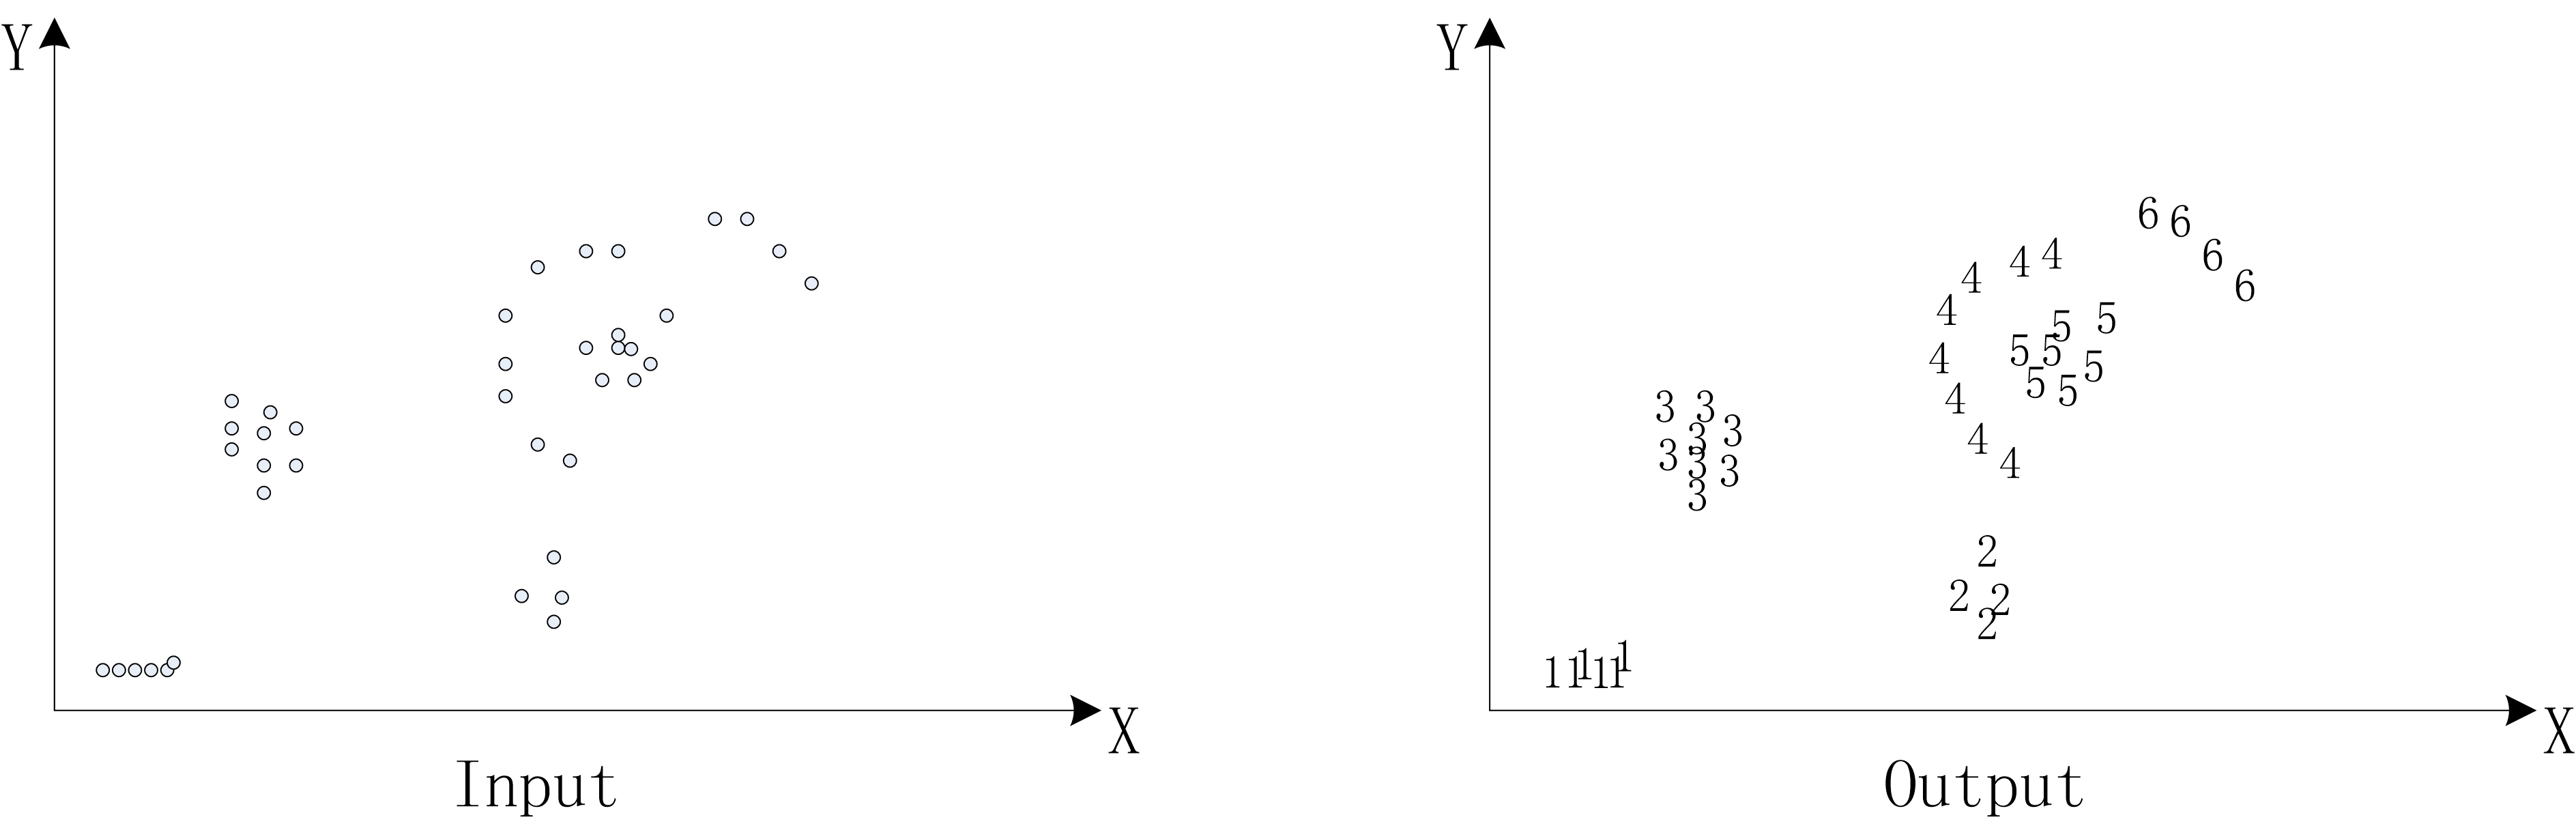
\includegraphics[width=300pt]{../images/clustering.jpg}
    \caption{An example of data clustering}
    \label{Fig:clustering}
\end{figure}
	
Hierarchical clustering algorithms are either top-down or bottom-up. Bottom-up algorithms treat each data as a singleton cluster at the outset and then successively merge (or agglomerate) pairs of clusters until all clusters have been merged into a single cluster that contains all data. Bottom-up hierarchical clustering is therefore called hierarchical agglomerative clustering. Top-down clustering requires a method for splitting a cluster. It proceeds by splitting clusters recursively until individual datum is reached\cite{manning2008introduction}.
% I don't really know what we're going to have the experimenter do yet.
% While performing experiments
% in this lab module, you, the experimenter, will learn how to make slight
% modifications to the basic search algorithm to progress between the different
% search types.
\subsubsection{An incremental conceptual clustering algorithm: COBWEB}

\paragraph{Conceptual Clustering}
Conceptual clustering is closely related to data clustering, however, it is distinguished from ordinary data clustering by generating a concept description for each generated class. In conceptual clustering, it is not only the inherent structure of the data that drives cluster formation, but also the description language which is available to the learner. Thus, a statistically strong grouping in the data may fail to be extracted by the learner if the prevailing concept description language is incapable of describing that particular regularity\cite{wikiconceptualclustering}. 

Conceptual clustering algorithms are generally used in situations where we may not have all the data when we want to start organizing our findings. The main purpose of the conceptual clustering algorithm is to allow for data elements to be organized in relation to each other as more data becomes available.

In most implementations, the description language has been limited to feature conjunction, however, in COBWEB, the feature language is probabilistic.

\paragraph {Incremental Clustering}
Incremental clustering is based on the assumption that it is possible to consider patterns one at a time and assign them to existing clusters. A typical incremental clustering algorithm is described as below\cite{jain1999data}:
\begin{itemize}\setlength{\itemsep}{0.01pt}
\item Assign the first data item to a cluster;
\item Consider the next data item. Either assign this item to one of the existing clusters or assign it to a new cluster. This assignment is done based on some criterion, e.g. the distance between the new item and the existing cluster centroids.
\item Repeat the second step till all the data items are clustered.
\end{itemize}

\paragraph {COBWEB}
The COBWEB conceptual clustering algorithm\cite{fisher1987knowledge} updates the tree (relation of all existing data elements) in accordance with new data that comes in. The tree this algorithm creates is devised in such a way that any \emph{frontier node} is a data element and any \emph{interior node} is a class which is a general representation of all of its children.

% Add picture of classes versus data elements in a tree.
The simplest way of thinking of the COBWEB conceptual clustering algorithm is in terms of a child boy cleaning up his toys (assuming he's only paying attention to the toys he has already organized). Say a child picks up a firetruck first, so he puts the firetruck in its own bin, simply because no bin is in use yet. Then he picks up a bouncy ball. This toy doesn't seem to relate to the firetruck at all, so the child decides to put the bouncy ball in a separate bin from the firetruck. The next toy the child picks up is a racecar. So at this point the child can choose to put the racecar in its own bin, or in the same bin as the firetruck since the racecar and firetruck have a lot in common. The child decides to put the racecar in the same bin as the firetruck because they have enough similarities to share a bin. This is the general concept of the COBWEB conceptual clustering algorithm. As data is brought in, decisions are made.

\subparagraph {Category Utility}
The first step of the COBWEB conceptual clustering algorithm is to determine the best spot for the new data element in the existing tree. That is, to determine which class the new data element fits into best. But one thing to note is that there are situations when the best option is to treat the new data element as its own entity and place it directly under the root node, rather than add it to an existing class.

But once a data element has been added to a class, there may be sub-classes into which it might fit better than the class it is currently assigned to. So in order to determine the best place for a new data element, the algorithm could possibly have to traverse all the way down to a class consisting of \emph{only} frontier nodes.

The next question is, how do we know which spot is \lq\lq{best}\rq\rq for a new element? This is determined by the \emph{categorical utility}\cite{gluck1985information} of adding the new data element to a certain spot in the tree. Category utility can be viewed as a function that rewards traditional virtues held in clustering generally--similarity of objects within the same class and dissimilarity of objects in different classes\cite{fisher1987knowledge}:

\begin{itemize}\setlength{\itemsep}{0.01pt}
\item Intra-class similarity is reflected by conditional probability: $P(A_i=V_{ij}\left|C_k\right.)$, where $A_i$ denotes an attribute, $V_{ij}$ denotes an attribute value, $C_k$ denotes a class. The larger this probability, the greater proportion of class members sharing the value and the more predictable the value is of class members\cite{fisher1987knowledge}.
\item Inter-class similarity is a function of $P(C_k|A_i=V_{ij})$. The larger this probability, the fewer the objects in contrasting classes that share this value and the more predictive the value is of the class\cite{fisher1987knowledge}.
\end{itemize}

Based on the intra-class and inter-class similarity, for a partition $\{C_1, C_2,...,C_n\}$ which is a set of mutually exclusive classes, the following equation $$E_1=\sum_{k=1}^{n}\sum_{i}\sum_{j}P(A_i=V_{ij})P(C_k|A_i=V_{ij})P(A_i=V_{ij}\left|C_k\right.)$$ overall measures the partition quality, where the probability $P(A_i=V_{ij})$ weights the importance of the individual attribute value. $E_1$ indicates that it is more important to increase the class-conditioned predictability and predictiveness of frequently occurring values than for infrequently occurring ones\cite{fisher1987knowledge}.

According to Bayes Rule, $ P(A_i=V_{ij})P(C_k|A_i=V_{ij})=P(C_k)P(A_i=V_{ij}|C_k)$. By substituting to $E_{1}$, we will get:$$E_1=\sum_{k=1}^{n}P(C_k)\sum_i \sum_jP(A_i=V_{ij}\left|C_k\right.)^2$$ which is the ability to correctly guess the attributes of an object in a certain class. 

Finally, category utility is defined by Cluck and Corter as the increase in the expected number of attribute values that can be correctly guessed $P(C_k)\sum_i \sum_jP(A_i=V_{ij}\left|C_k\right.)^2$ over the expected
number of correct guesses without such knowledge $\sum_i \sum_jP(A_i=V_{ij})^2$\cite{fisher1987knowledge}:
\begin{equation*}
\label{eq:cu}
%\text{Category Utility}
CU=\frac{\sum_{k=1}^{n}P(C_k)\left[\sum_i \sum_jP(A_i=V_{ij}\left|C_k\right.)^2-\sum_i \sum_jP(A_i=V_{ij})^2\right]}{n}
\end{equation*}

Here is an example: if a class has 8 green balls and 2 red balls and a different class has 4 green squares and 7 blue squares and the new element is a blue ball, the new blue ball will be placed in the first class according to the category utility since the CU value for this partition is the highest.
\begin{table}[!ht]
\ttabbox{\caption{Table of Classes}}{
\centering
\begin{minipage}{0.45\textwidth}
\begin{tabular}{l l l}\hline
\textbf{ } & \textbf{Class 1} & \textbf{ }\\
\textbf{A1} & \textbf{A2} & \textbf{Number}\\\hline
Green & Ball & 8 \\
Red & Ball & 2 \\\hline
\end{tabular}
\end{minipage}
\hfil
\begin{minipage}{0.45\textwidth}
\begin{tabular}{l l l}\hline
\textbf{ } & \textbf{Class 2} & \textbf{ }\\
\textbf{A1} & \textbf{A2} & \textbf{Number}\\\hline
Green & Square & 4 \\
Blue & Square & 7 \\\hline
\end{tabular}
\label{tab:label}
\end{minipage}}
\end{table}
% Check the above example

By the definition above, we can say in this example, there are two classes $C_1$ and $C_2$ (shown in Table \ref{tab:label}), and two attributes \emph{color} and \emph{shape} with five attribute values which are: $$A_1=\{\text{color}|V_{11}=\text{Green},V_{12}=\text{Red}, V_{13}=\text{Blue}\}$$$$A_2=\{\text{shape}|V_{21}=\text{Ball}, V_{22}=\text{Square}\}$$

First, if we place the new element \{Blue Ball\} in Class 1(shown in Table \ref{tab:label2}), we can calculate CU for the current partition. The probability for $C_1$ is $$P(C_1)=\frac{8+2+1}{8+2+1+4+7}=0.5$$ and the probability for $C_2$ is $$P(C_2)=\frac{4+7}{8+2+1+4+7}=0.5$$ 
The expected number of attribute values that can be correctly guessed given $C_1$ is: 
\begin{equation*}
\begin{aligned}
&\sum_{i=1}^{2} \sum_{j=1}^{3}P(A_i =V_{ij}\left|C_1\right.)^2\\
=&(\frac{8}{8+2+1})^2+(\frac{2}{8+2+1})^2+(\frac{1}{8+2+1})^2+(\frac{8+2+1}{8+2+1})^2+0\\
=&1.5702
\end{aligned}
\end{equation*} % % % too long to put in one line
and the expected number of attribute values that can be correctly guessed given $C_2$ is: $$\sum_{i=1}^{2} \sum_{j=1}^{3}P(A_i=V_{ij}\left|C_2\right.)^2=(\frac{4}{4+7})^2+0+(\frac{7}{4+7})^2+0+(\frac{4+7}{4+7})^2=1.5372$$
%\begin{equation*}
%\begin{aligned}
%\end{aligned}
%\end{equation*} 
The expected number of attribute values that can be correctly guessed without any category knowledge is: $$\sum_{i=1}^{2} \sum_{j=1}^{3}P(A_i=V_{ij})^2=(\frac{8+4}{8+2+1+4+7})^2+(\frac{2}{22})^2+(\frac{1+7}{22})^2+(\frac{8+2+1}{22})^2+(\frac{4+7}{22})^2=0.9380$$ 
Thus, we can get CU for adding the new element to the Class 1: $$CU_1=\frac{0.5\times(1.5702-0.9380)+0.5\times(1.5372-0.9380)}{2}=0.30785$$

\begin{table}[!ht]
\ttabbox{\caption{Table of Classes by adding the new element in $C_1$}}{
\centering
\begin{minipage}{0.45\textwidth}
\begin{tabular}{l l l}\hline
\textbf{ } & \textbf{$C_1$} & \textbf{ }\\\hline
\textbf{A1} & \textbf{A2} & \textbf{Number}\\
\hline
Green & Ball & 8 \\
Red & Ball & 2 \\
Blue & Ball & 1\\\hline
\end{tabular}
\end{minipage}
\hfil
\begin{minipage}{0.45\textwidth}
\begin{tabular}{l l l}\hline
\textbf{ } & \textbf{$C_2$} & \textbf{ }\\\hline
\textbf{A1} & \textbf{A2} & \textbf{Number}\\\hline
Green & Square & 4 \\
Blue & Square & 7 \\\hline
\end{tabular}
\label{tab:label2}
\end{minipage}}
\end{table}

Second, in the same manner, we can also get CU for adding the new element to the Class 2(shown in Table \ref{tab:label3}), which is: $$CU_2=\frac{\frac{10}{22}\times(1.68-0.9380)+\frac{12}{22}\times(1.4028-0.9380)}{2}=0.2954$$

\begin{table}[!ht]
\ttabbox{\caption{Table of Classes by adding the new element in $C_2$}}
{
\centering
\begin{minipage}{0.45\textwidth}
\begin{tabular}{l l l}\hline
\textbf{ } & \textbf{$C_1$} & \textbf{ }\\\hline
\textbf{A1} & \textbf{A2} & \textbf{Number}\\
\hline
Green & Ball & 8 \\
Red & Ball & 2 \\
\hline
\end{tabular}
\end{minipage}
\hfil
\begin{minipage}{0.45\textwidth}
\begin{tabular}{l l l}\hline
\textbf{ } & \textbf{$C_2$} & \textbf{ }\\\hline
\textbf{A1} & \textbf{A2} & \textbf{Number}\\\hline
Green & Square & 4 \\
Blue & Square & 7 \\
Blue & Ball & 1\\\hline
\end{tabular}
\label{tab:label3}
\end{minipage}}
\end{table}

Last, besides the possibility that placing the new element in an existing class, there is a chance for the new element generate a new class by itself. In the same manner, we can further calculate CU for generating a new class for the new element(shown in Table \ref{tab:label4}), which is $$CU_3=\frac{\frac{10}{22}\times(1.68-0.9380)+\frac{11}{22}\times(1.5372-0.9380)+\frac{1}{22}\times(2-0.9380)}{3}=0.2284$$ 
\begin{table}[!ht]
\ttabbox{\caption{Table of Classes by generating a new class with the new element}}
{
\centering
\begin{minipage}{0.35\textwidth}
\begin{tabular}{l l l}\hline
\textbf{ } & \textbf{$C_1$} & \textbf{ }\\\hline
\textbf{A1} & \textbf{A2} & \textbf{Number}\\
\hline
Green & Ball & 8 \\
Red & Ball & 2 \\
\hline
\end{tabular}
\end{minipage}
\hfil
\begin{minipage}{0.35\textwidth}
\begin{tabular}{l l l}\hline
\textbf{ } & \textbf{$C_2$} & \textbf{ }\\\hline
\textbf{A1} & \textbf{A2} & \textbf{Number}\\\hline
Green & Square & 4 \\
Blue & Square & 7 \\
\hline
\end{tabular}
\end{minipage}
\hfil
\begin{minipage}{0.35\textwidth}
\begin{tabular}{l l l}\hline
\textbf{ } & \textbf{$C_3$} & \textbf{ }\\\hline
\textbf{A1} & \textbf{A2} & \textbf{Number}\\\hline
Blue & Ball & 1\\\hline
\end{tabular}
\label{tab:label4}
\end{minipage}}
\end{table}

\subparagraph {COBWEB Operations}
The COBWEB algorithm constructs a classification tree incrementally by inserting the objects into the tree one by one. When inserting an new object into the classification tree, the COBWEB algorithm descend the tree along a path of \lq\lq{best matching nodes}\rq\rq\cite{luger2011artificial} and performing one of the following operations at each level\cite{fisher1987knowledge}:
\begin{itemize}\setlength{\itemsep}{0.01pt}
\item Create the new object as a new class
\item Add the new object to an existing class with the highest CU
\item Merge two classes into a single class, or
\item Split a class into several classes
\end{itemize}

In the following, we will demonstrate each operation by taking the example of animal descriptions from the reference\cite{fisher1987knowledge}. 
\begin{table}[!ht]
\ttabbox{\caption{Table of Animal Descriptions}}
{
\centering
\begin{tabular}{l l l l l}\hline
\textbf{Name} & \textbf{Body Cover} & \textbf{Heart Chamber} & \textbf{Body Temp} & \textbf{Fertilization}\\\hline
\textbf{Mammal} & \textbf{Hair} & \textbf{4} & \textbf{Regulated} & \textbf{Internal}\\
\textbf{Bird} & \textbf{Feathers} & \textbf{4} & \textbf{Regulated} & \textbf{Internal}\\
\textbf{Reptile} & \textbf{Cornified-skin} & \textbf{Imperfect 4} & \textbf{Unregulated} & \textbf{Internal}\\
\textbf{Amphibian} & \textbf{Moist-skin} & \textbf{3} & \textbf{Unregulated} & \textbf{External}\\
\textbf{Fish} & \textbf{Scales} & \textbf{2} & \textbf{Unregulated} & \textbf{External}\\
\hline
\end{tabular}
\label{tab:animal}}
\end{table}

Suppose the current classification tree has been built by \lq{\emph{fish}}\rq and  \lq{\emph{amphibian}}\rq from Table\ref{tab:animal}. The tree is shown in Figure\ref{Fig:animaltree}. Listed with each box(node) are the probability of the class and the conditional probabilities of attribute values given the current class.
\begin{figure}[!ht]
    \centering
    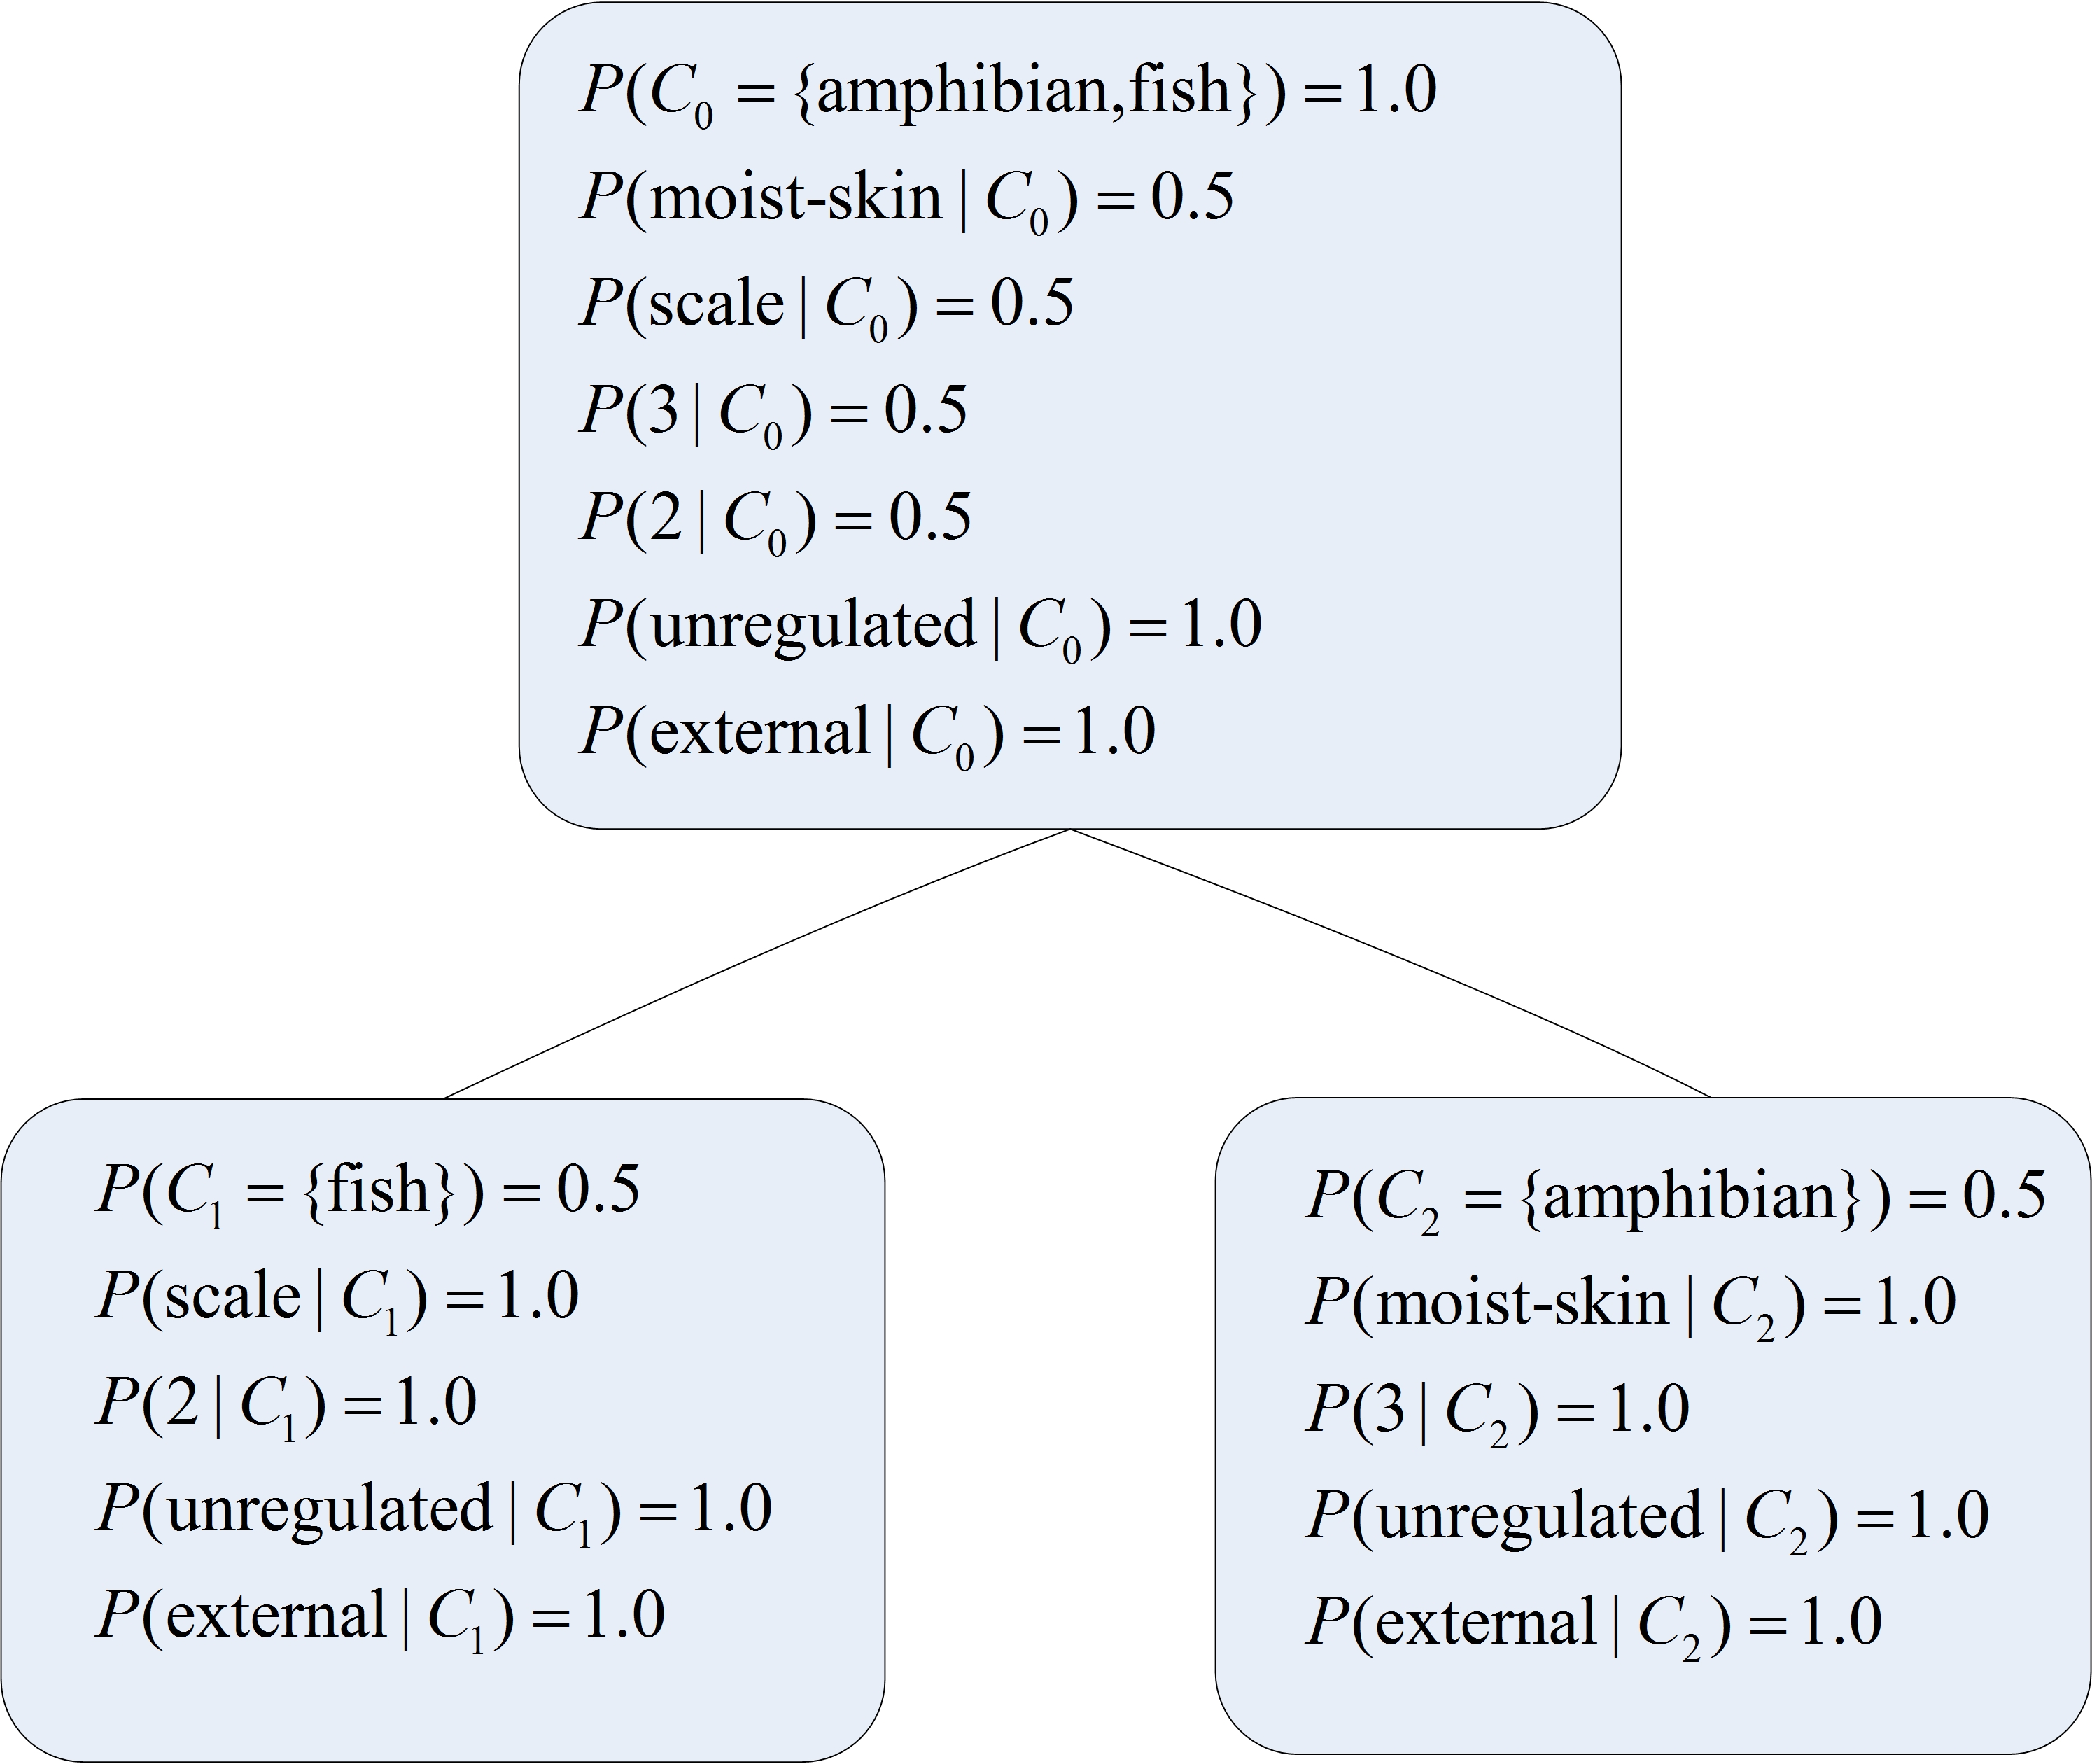
\includegraphics[width=200pt]{../images/animaltree.jpg}
    \caption{Classification tree built by \emph{fish} and \emph{amphibian}}
    \label{Fig:animaltree}
\end{figure}

\textbf{\emph{Creating the new object as a new class}} If the new element \lq{\emph{mammal}}\rq comes, by calculating category utility for classifying \lq{\emph{mammal}}\rq with the existing class \lq{\emph{fish}}\rq, CU for classifying \lq{\emph{mammal}}\rq with the other existing class \lq{\emph{amphibian}}\rq, and CU for creating a new class by \lq{\emph{mammal}}\rq only, we will know where we should put the new element. It turns out that creating a new singleton class with \lq{\emph{mammal}}\rq yields a better partition than adding the element to either of the existing classes. Correspondingly, the tree will transit from the above form to the Figure \ref{Fig:animaltree_create}.
\begin{figure}[!ht]
    \centering
    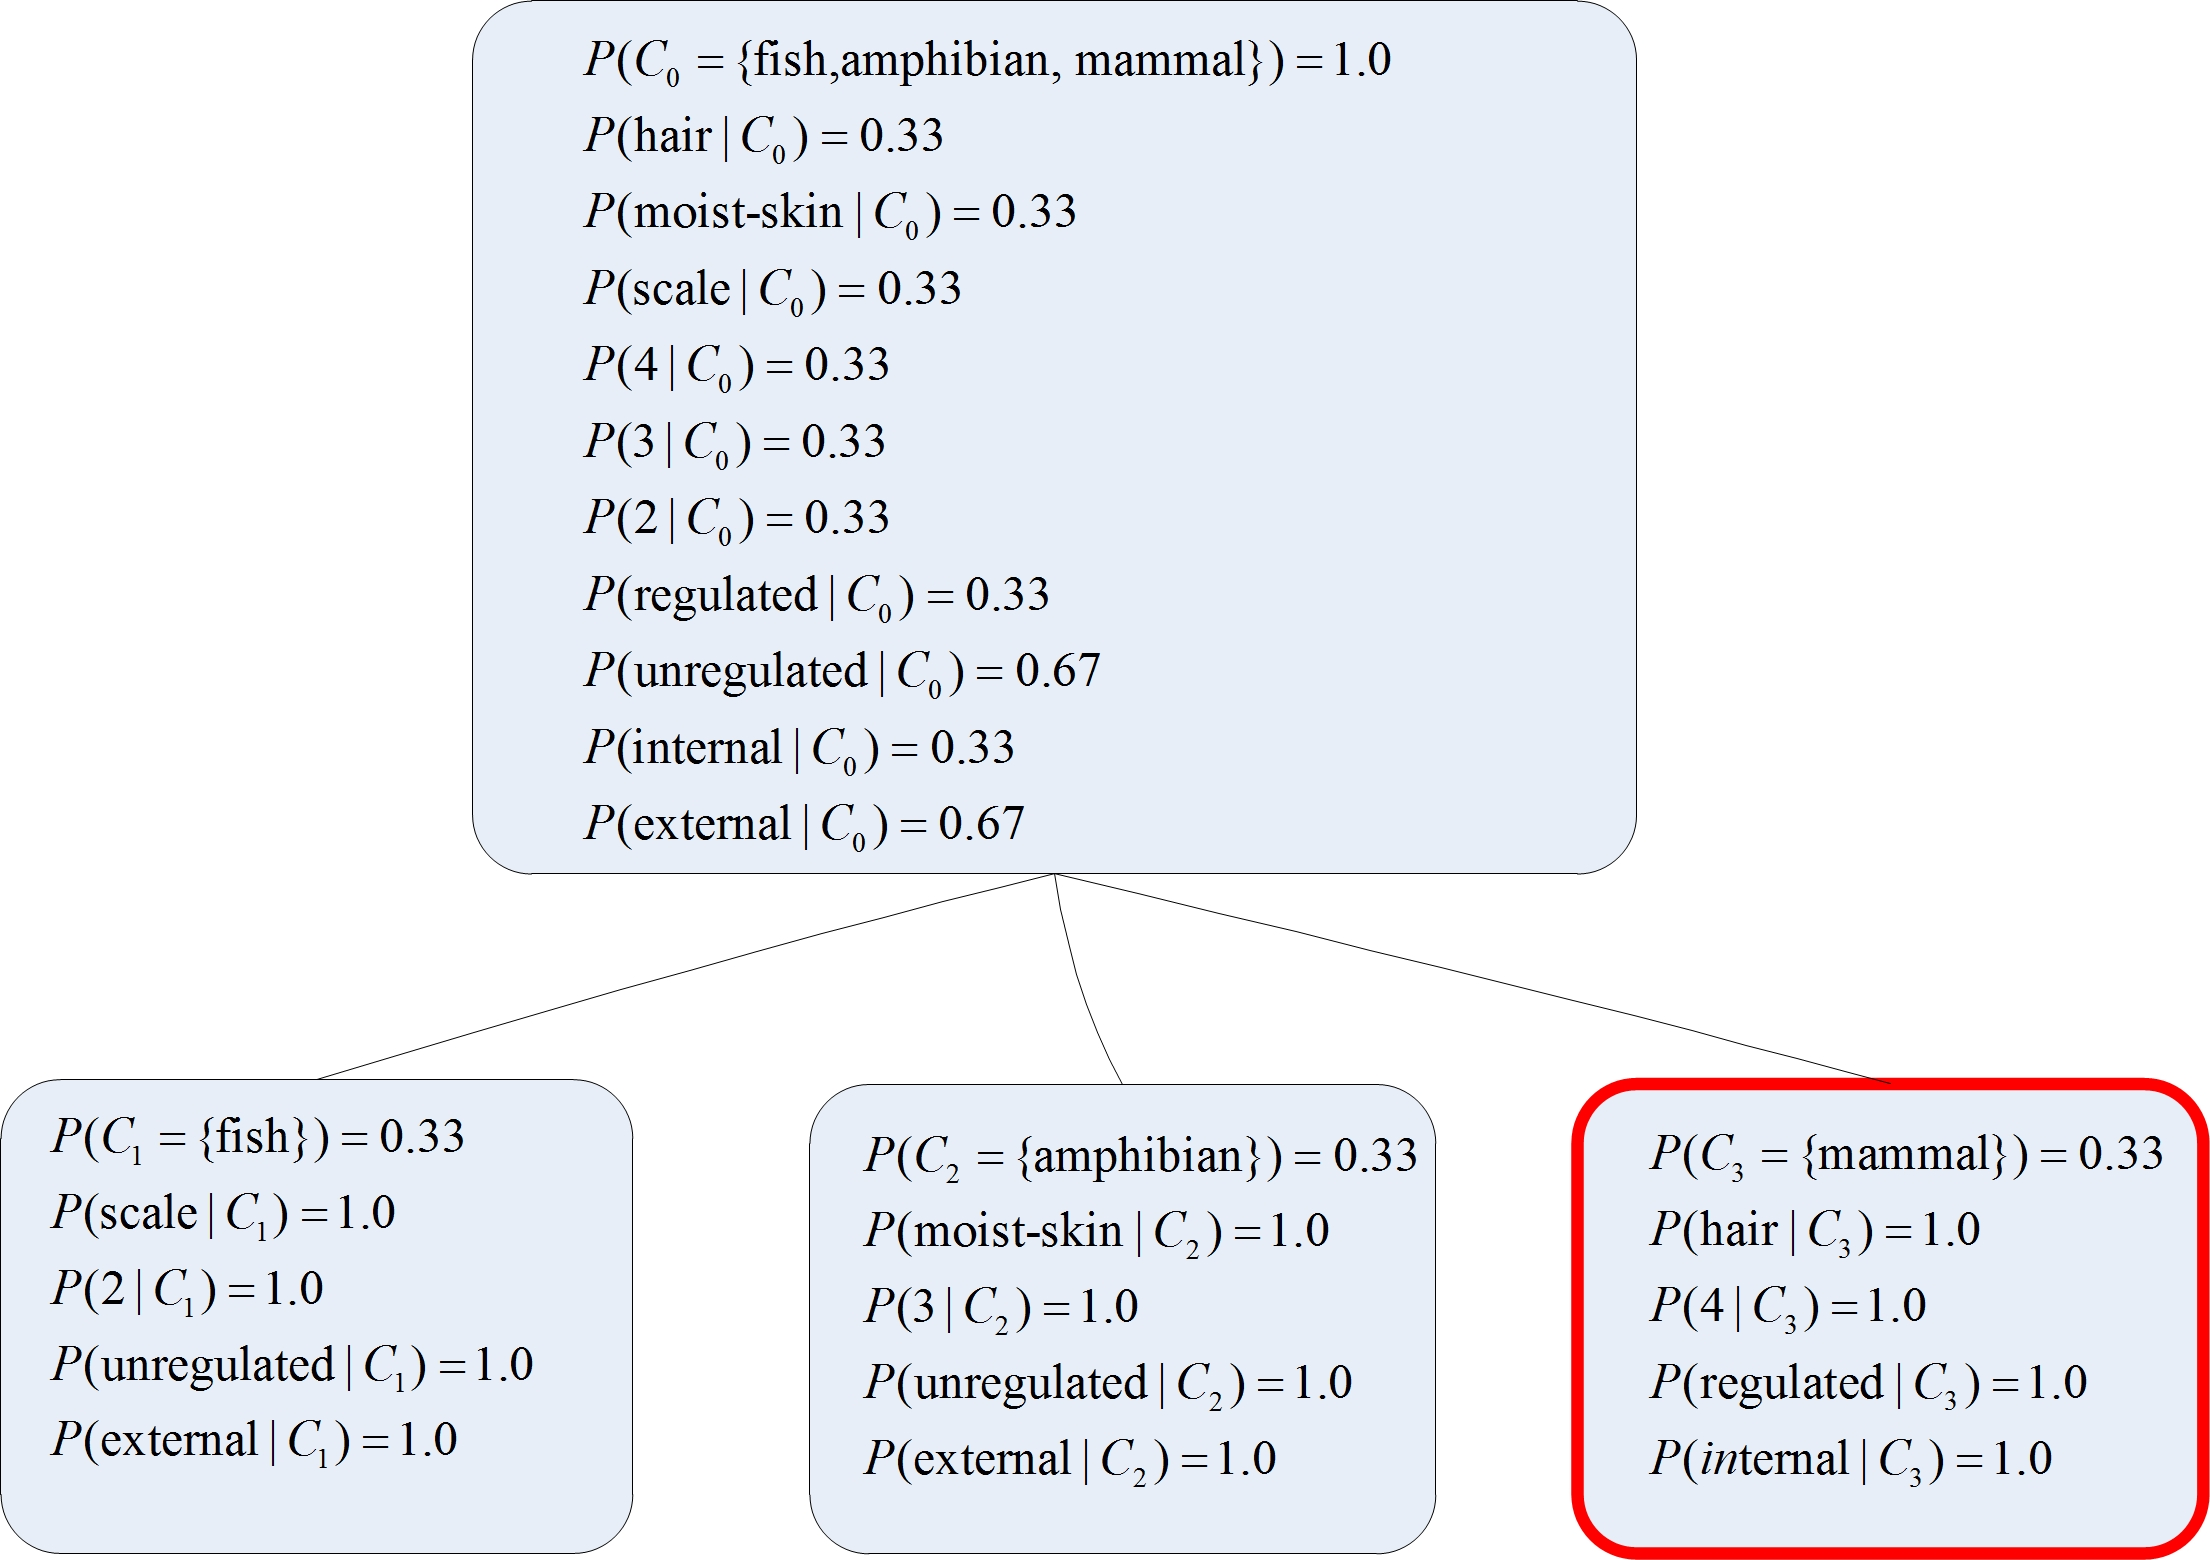
\includegraphics[width=300pt]{../images/animaltree_create.jpg}
    \caption{Adding '\emph{mammal}' to the existing classification tree}
    \label{Fig:animaltree_create}
\end{figure}

\textbf{\emph{Adding the new object to an existing class with the highest CU}} Next, if another new element \lq{\emph{bird}}\rq comes, based on CU, it's easy to know the new element \lq{\emph{bird}}\rq should be added to the existing class \lq{\emph{mammal}}\rq. Since the node \lq{\emph{mammal}}\rq in Figure\ref{Fig:animaltree_create} is a leaf, incorporation of \lq{\emph{bird}}\rq involves expanding the leaf to accommodate the new element \lq{\emph{bird}}\rq, as well as the previously classified one \lq{\emph{mammal}}\rq. The classification tree after \lq{\emph{bird}}\rq is added is shown in Figure\ref{Fig:animaltree_add}.
\begin{figure}[!ht]
    \centering
    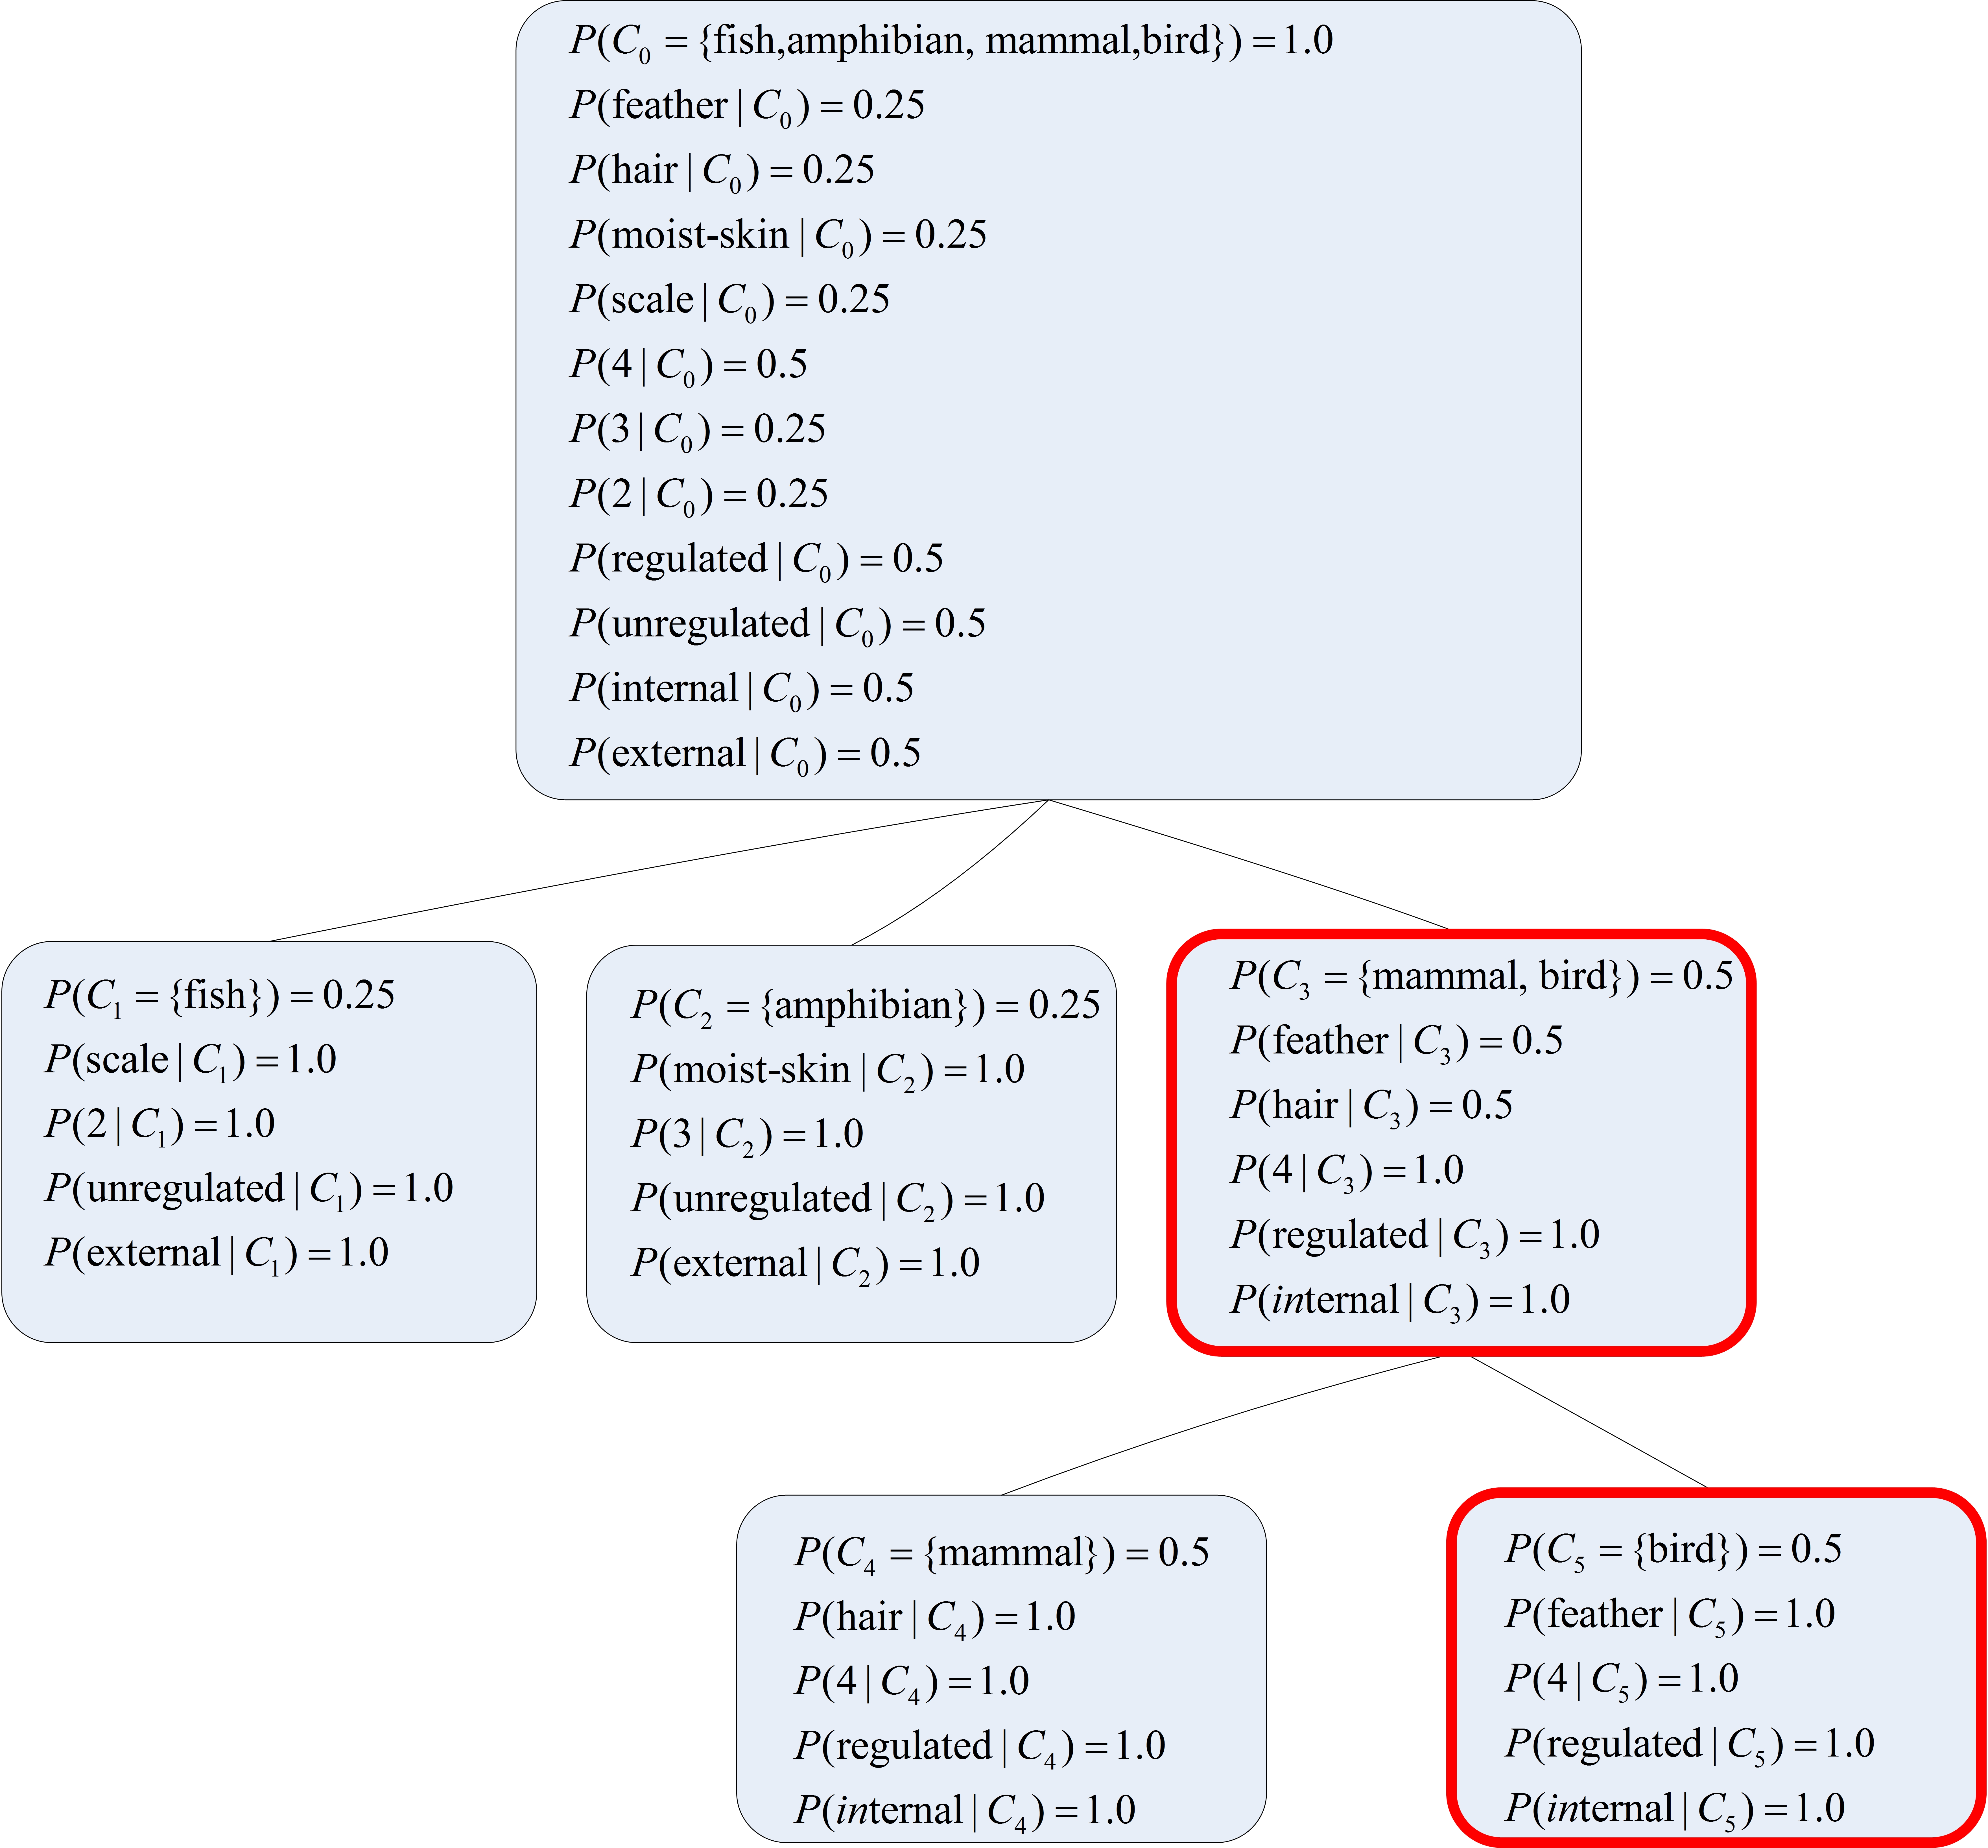
\includegraphics[width=300pt]{../images/animaltree_add.jpg}
    \caption{Adding \lq{\emph{bird}}\rq to the existing classification tree}
    \label{Fig:animaltree_add}
\end{figure}

While the two operations, creating the new object as a new class and adding the new object to an existing class, are effective in many cases, by themselves they are very sensitive to the ordering of initial input. To guard against the effects of initially skewed data, COBWEB includes operations for node merging and splitting. When adding a new object, only the two classes with best CU are considered for merging\cite{fisher1987knowledge}. 

\textbf{\emph{Merging two classes into a single class}} Then, if another element \lq{\emph{fish}}\rq comes, classes $C_1$ and $C_2$ in the Figure \ref{Fig:animaltree_add} are identified as the best and second best hosts for the new element \lq{\emph{fish}}\rq. Merging $C_1$, $C_2$ and the new element \lq{\emph{fish}}\rq results in a partition superior to that obtained by incorporating the new element in the best host $C_1$. The classification tree spanned from Figure \ref{Fig:animaltree_add} is shown in the Figure \ref{Fig:animaltree_merge}.
\begin{figure}[!ht]
    \centering
    \includegraphics[width=300pt]{../images/animaltree_merge.jpg}
    \caption{Adding \lq{\emph{fish}}\rq to the existing classification tree}
    \label{Fig:animaltree_merge}
\end{figure}

\textbf{\emph{Splitting a class into several classes}} Splitting is the inverse operation of merging. Splitting is considered only for the children of the best host among the existing categories. A node of a partition (of n nodes) may be deleted and its children promoted, resulting in a partition of n + m - 1 nodes, where the deleted node had m children\cite{fisher1987knowledge}. An example of splitting is shown in Figure\ref{Fig:split}. 

\begin{figure}[!ht]
    \centering
    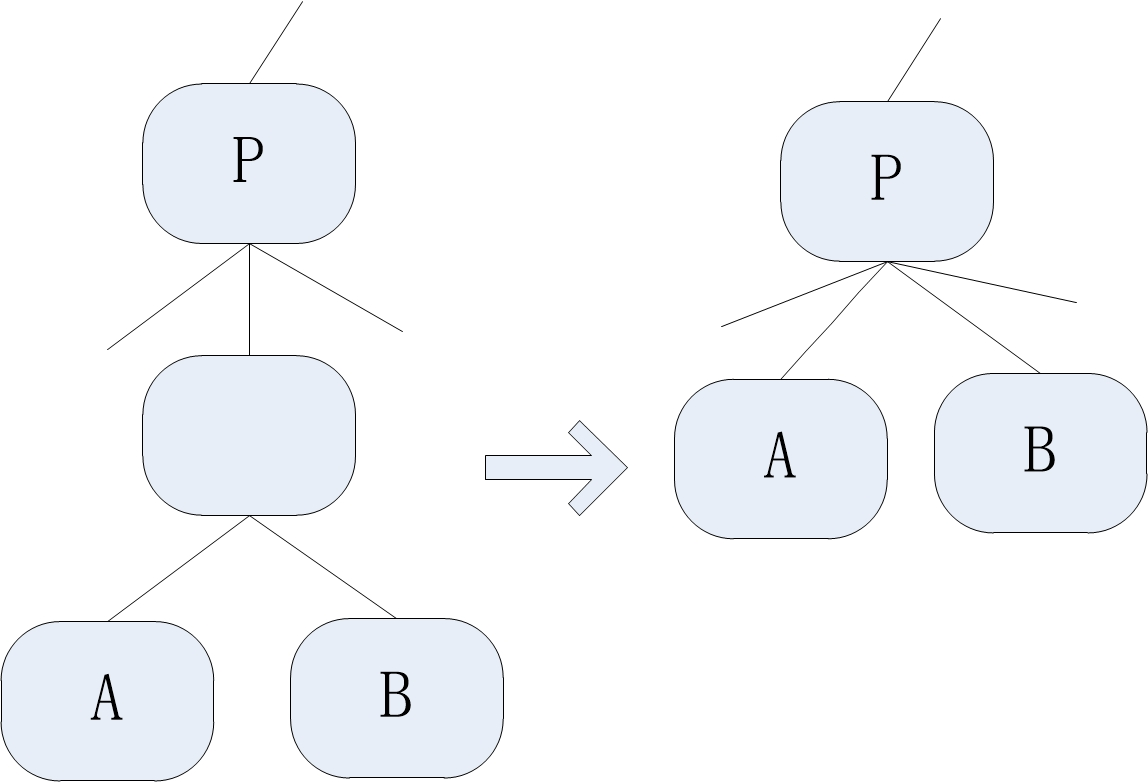
\includegraphics[width=200pt]{../images/split.jpg}
    \caption{An example of node splitting}
    \label{Fig:split}
\end{figure}

\subparagraph {COBWEB Algorithm}
We have detailed the evaluation measure of COBWEB--category utility, and the four operations involved in COBWEB algorithm. The structure of COBWEB algorithm can be summarized as:
\begin{itemize}\setlength{\itemsep}{0.01pt}
\item Tentatively add to each existing portion
\item Calculate CU of each
\item Calculate CU for adding the new object directly to the root
\item Add the new object to the child of the root with the highest CU
\item As with all hill-climbing, presentation order determines initial tree structure
\item MERGE and SPLIT operators minimize the effect of input ordering, and improve partition quality.
\end{itemize}



%
% 2-Applications.tex
%
%  LaTeX source file for section 2 Applications for the Conceptual Clustering lab module of the TAILS project.
%

\section{Applications}
Conceptual clustering is widely used in our life. Learning itself is a kind of conceptual clustering. As a child grows up, he may learn to play toy blocks, count, recognize shapes and letters, he may learn maths, drawing, reading and writing, and later he may learn Artificial Intelligence, arts and English literature. Each time when a child learns something new, new knowledge will be stored in his knowledge base and relate to what he has already known or span a new space in his knowledge base. Similar knowledge is grouped together to form a category. As time goes by, the knowledge base broadens just like the classification tree spans. For example, when a student learns geometry in middle school, he may automatically add his previous experience with shapes to the new subject. Later when he learns architecture in college, he may probably reorganize his knowledge by adding geometry as the child node of architecture. Reference to Figure\ref{Fig:app1}. Those knowledge categories in mind help a person to respond to the problems from the outside world smoothly. For example, when the student participates a group project about designing a museum, he may need to search the related knowledge category in mind like architecture, recall related experience and finally reacts to the problem.

\begin{figure}[h!]
    \centering
    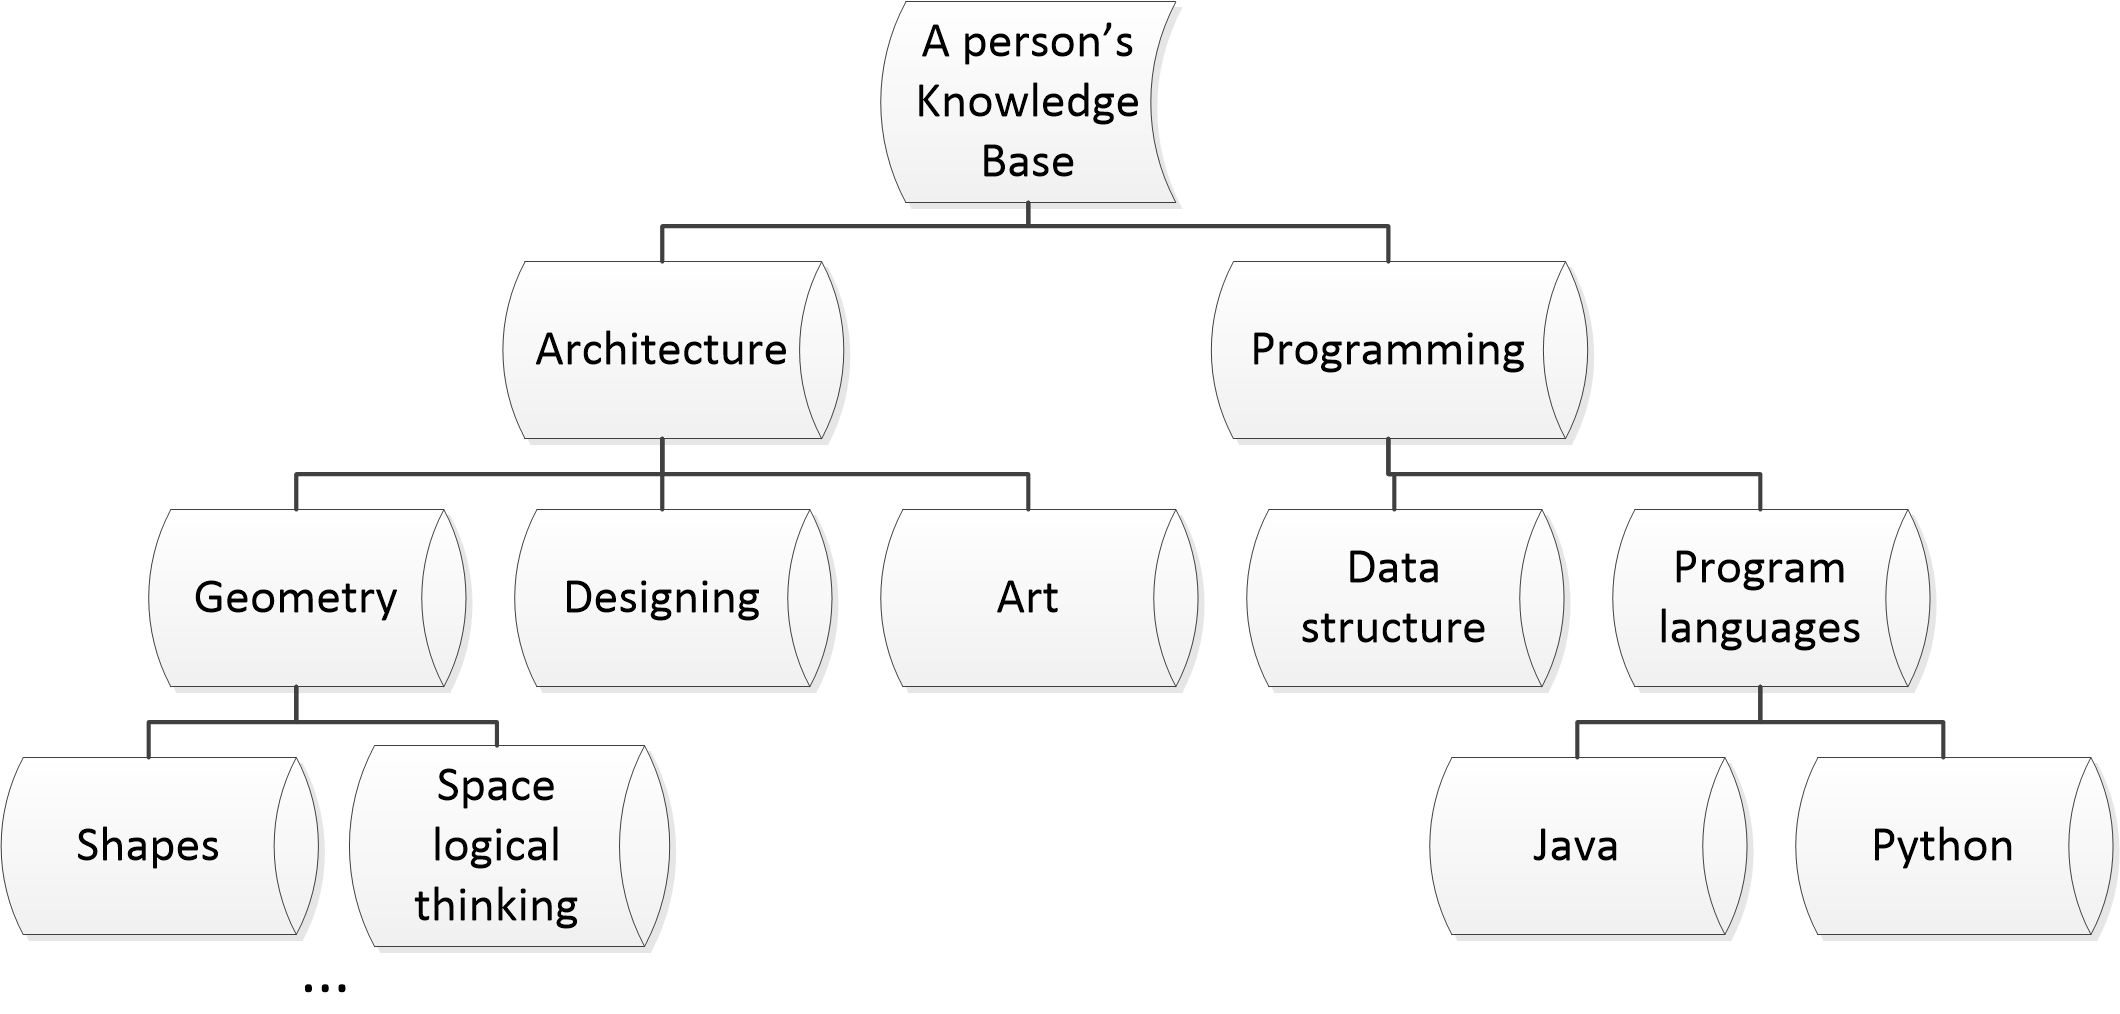
\includegraphics[width=300pt]{../images/app1.jpg}
    \caption{An example of classification tree for a person's knowledge base}
    \label{Fig:app1}
	\end{figure}
	
Another possible example is that zoologist finds some new species from a isolated island. He may need to examine the new species from the structure or gene to decide if the new species belongs to any known class or it is a new class. The classification tree is shown in Figure \ref{Fig:app2}
\begin{figure}[h!]
    \centering
    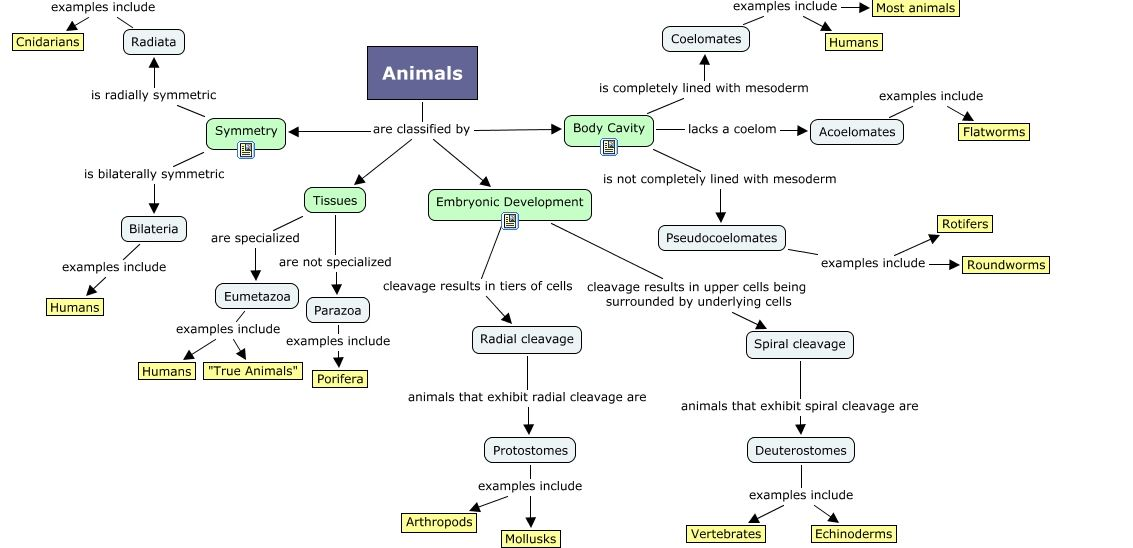
\includegraphics[width=400pt]{../images/app2.jpg}
    \caption{The classification tree for animals\cite{newyork}}
    \label{Fig:app2}
	\end{figure}



%
% 3-input-process-output.tex
%
%  LaTeX source file for section 3 Input-Process-Output for the Conceptual Clustering lab module of the TAILS project.
%

\section{Input-Process-Output}

\subsection{Input}
The input to this laboratory includes user-defined objects with various attributes and values. Let's say if we want to cluster different geometric figures, we may describe them  in multiple aspects, like shape, color or size. It's possible to have triangle, circle or rectangle. So here, \lq\lq{shape}\rq\rq, \lq\lq{color}\rq\rq and \lq\lq{size}\rq\rq are the attributes, and \lq\lq{triangle}\rq\rq, \lq\lq{circle}\rq\rq and \lq\lq{rectangle}\rq\rq are the attribute values for the attribute \lq\lq{shape}\rq\rq. The inputs for attributes and their values should be in the form of words only and it's case-insensitive. The input interface is shown in Figure \ref{Fig:intf1}. 
  \begin{figure}[h!]
     \centering
     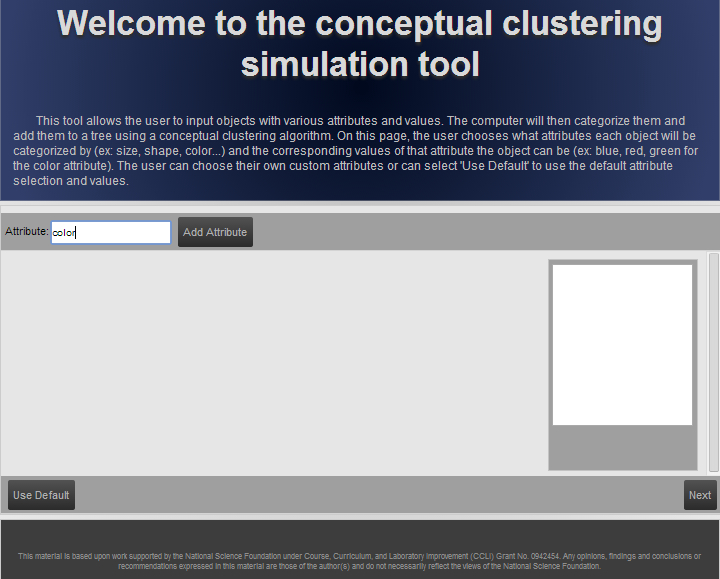
\includegraphics[width=300pt]{../images/interface1.jpg}
     \caption{The User Interface of Conceptual Clustering : Users can  input custom data either by the browser input or uploading from a file, or users can use the default setting}
     \label{Fig:intf1}   
     \end{figure}

If users want to input custom data, the tool allows for inputting data by the browser input or loading from a file. Using the browser input, users need to type in attribute names and their values accordingly. An attribute name should be typed in first in the attribute box and then click the \lq\lq{Add Attribute}\rq\rq button. The newly added attribute will be displayed under the input box. Moving the mouse on the attribute, the input box for attribute values will show up. Next, various values for the specific attribute can be typed in with the form of word only. An example is shown in Figure \ref{Fig:intf2}. 
 \begin{figure}[h!]
        \centering
        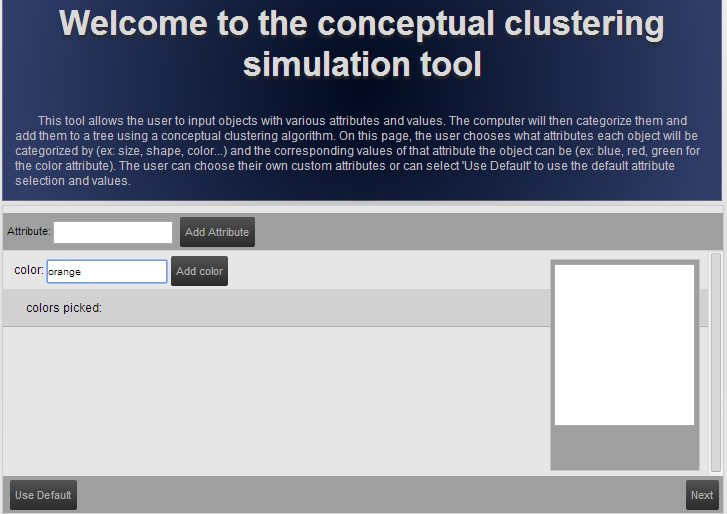
\includegraphics[width=300pt]{../images/interface2.jpg}
        \caption{Input custom data by the browser input}
        \label{Fig:intf2}
    \end{figure}

Users may also choose to load attributes and values from other documents by the box on the right. An example is shown in Figure \ref{Fig:intf2_loadfile}. These attributes are copied from a text file, which are  \lq\lq{color,size\#orange,blue,red\#large,small\#}\rq\rq. Clicking \lq\lq{Load Attributes}\rq\rq button, the custom data will be inputted. Whatever is loaded, the contents should follow the following rules:
\begin{enumerate}\renewcommand{\labelenumi}{(\theenumi)}\setlength{\itemsep}{0.05pt}
\item Attribute or values should be in the format of word only; 
\item Any attributes or values should be separated by a comma without a space;
\item Each line is separated by a pound sign \lq\lq{\#}\rq\rq;
\item The contents in first line will be identified as the attributes and the other lines will be recognized as the attribute values for each attribute defined in the first line;
\item An \lq\lq{Enter}\rq\rq at the end of each line makes no difference.
\end{enumerate}  
 \begin{figure}[h!]
       \centering
       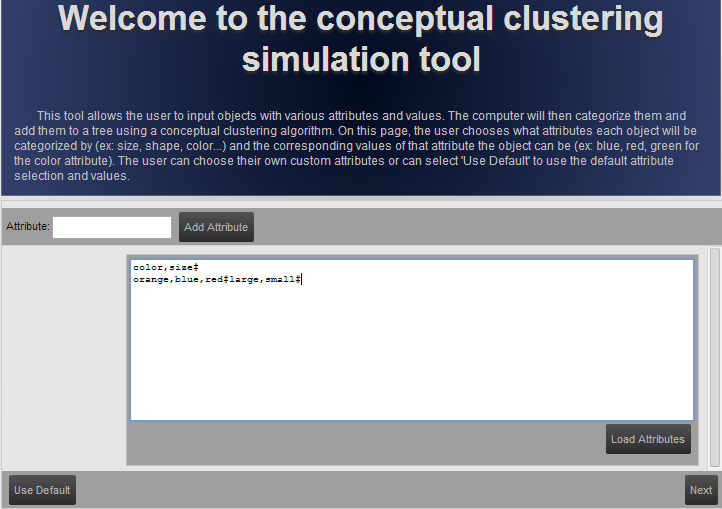
\includegraphics[width=300pt]{../images/interface2_loadfile.jpg}
       \caption{Input custom data by loading a file}
       \label{Fig:intf2_loadfile}
 \end{figure}  
 
Except for inputting custom attributes, users can click the \lq\lq{Use Default}\rq\rq button to use the default attribute selections and values. 	

\subsection {Process}
The simulation tool will display all the attributes and their values in the second interface and enable users to input different objects from the radio buttons. The tool will categorize the input objects and add them to a classification tree based on the COBWEB conceptual clustering algorithm. The second interface is shown in Figure\ref{Fig:intf3}. 
    
On the left, one or multiple objects can be added to generate the classification tree by selecting different attribute values and clicking \lq\lq{Add}\rq\rq or \lq\lq{Add Multiple}\rq\rq button. The dynamic graph of generating the classification tree will be displayed, showing how the clustering algorithm works. 
     
Moving the mouse on the node in the tree, the probabilistic concept label for this node will show up. The label includes the conditional probability for each attribute value given the current cluster, which corresponds to $P(A_i=V_{ij}\left|C_k\right.)$ and the percentage of the current cluster against the entire tree, which corresponds to $P(C_k)$ in the Category Utility function on Page 5. 

On the bottom of the visual window, every time a new object is added, there will be an explanation for what specific operation is carried out for the current step. Those operations are denoted as \lq\lq{Added node}\rq\rq, \lq\lq{Formed new subtree}\rq\rq, \lq\lq{Merged}\rq\rq and \lq\lq{Split}\rq\rq which correspond to the four COBWEB operations listed in Page 7.
    \begin{figure}[h!]
           \centering
           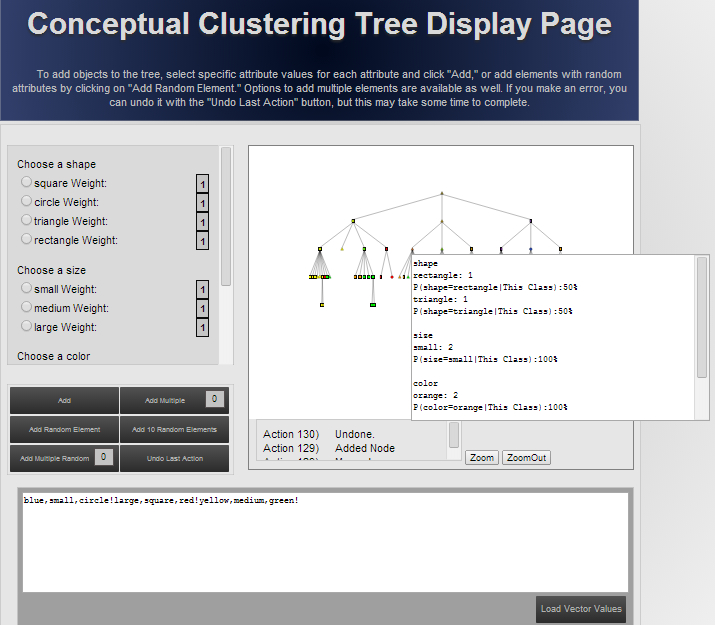
\includegraphics[width=300pt]{../images/interface3.jpg}
           \caption{The process of generating the clustering tree}
           \label{Fig:intf3}
     \end{figure}    
     
On the bottom of the tree display page, there is a input box allowing users to input objects by loading from other files. The format is the same as that for attribute, except that there should be an exclamation mark \lq\lq{!}\rq\rq separating the descriptions from one object to the next one. In the example shown in Figure \ref{Fig:intf3}, we copied \lq\lq{blue,small,circle!large,square,red!yellow,medium,green!}\rq\rq from a text file. By clicking \lq\lq{Load Vector Values}\rq\rq button, these objects will be added to the tree.

\subsection {Output}
The classification tree keeps spanning as long as more objects are added. The classification tree indicates the clusters for current input space. All the leaf nodes that share the same parent node is grouped into one cluster.
\subsection {Example}
 In this section, three experiments will be used to illustrate the effect of the input orders for the COBWEB algorithm. As we know, only one datum item is being considered at a time. The classification tree is sensitive to the input orders\cite{fisher1987knowledge}. The two operations merging and splitting are able to minimize the effect of the input orders but can not remove the effect.
 
 In order to observe the effect of the inputs orders, we carry out three experiments by using the same set of data in Table\ref{tab:inputseq}.
 \begin{table}[!ht]
 \ttabbox{\caption{Table of input data}}
 {
 \centering
 \begin{tabular}{l l l l l l l l}\hline
 \textbf{} & \textbf{shape} & \textbf{size} & \textbf{color}   & \textbf{} & \textbf{shape} & \textbf{size} & \textbf{color}\\\hline
 \textbf{1} & \textbf{square} & \textbf{large} & \textbf{blue}   & \textbf{6} & \textbf{circle} & \textbf{large} & \textbf{blue}\\
 \textbf{2} & \textbf{square} & \textbf{large} & \textbf{yellow} & \textbf{7} & \textbf{circle} & \textbf{large} & \textbf{yellow}\\
 \textbf{3} & \textbf{square} & \textbf{large} & \textbf{red}    & \textbf{8} & \textbf{circle} & \textbf{large} & \textbf{red}\\
 \textbf{4} & \textbf{square} & \textbf{large} & \textbf{orange} & \textbf{9} & \textbf{circle} & \textbf{large} & \textbf{orange}\\
 \textbf{5} & \textbf{square} & \textbf{large} & \textbf{green}  & \textbf{10} & \textbf{circle} & \textbf{large} & \textbf{green}\\
 \hline
 \end{tabular}
 \label{tab:inputseq}}
 \end{table}
 
 If we input the data with the sequence shown in the Table\ref{tab:inputseq}, the tree will be generated in the way shown in Figure\ref{Fig:inputseq1}. 
 \begin{figure}[h!]
            \centering
            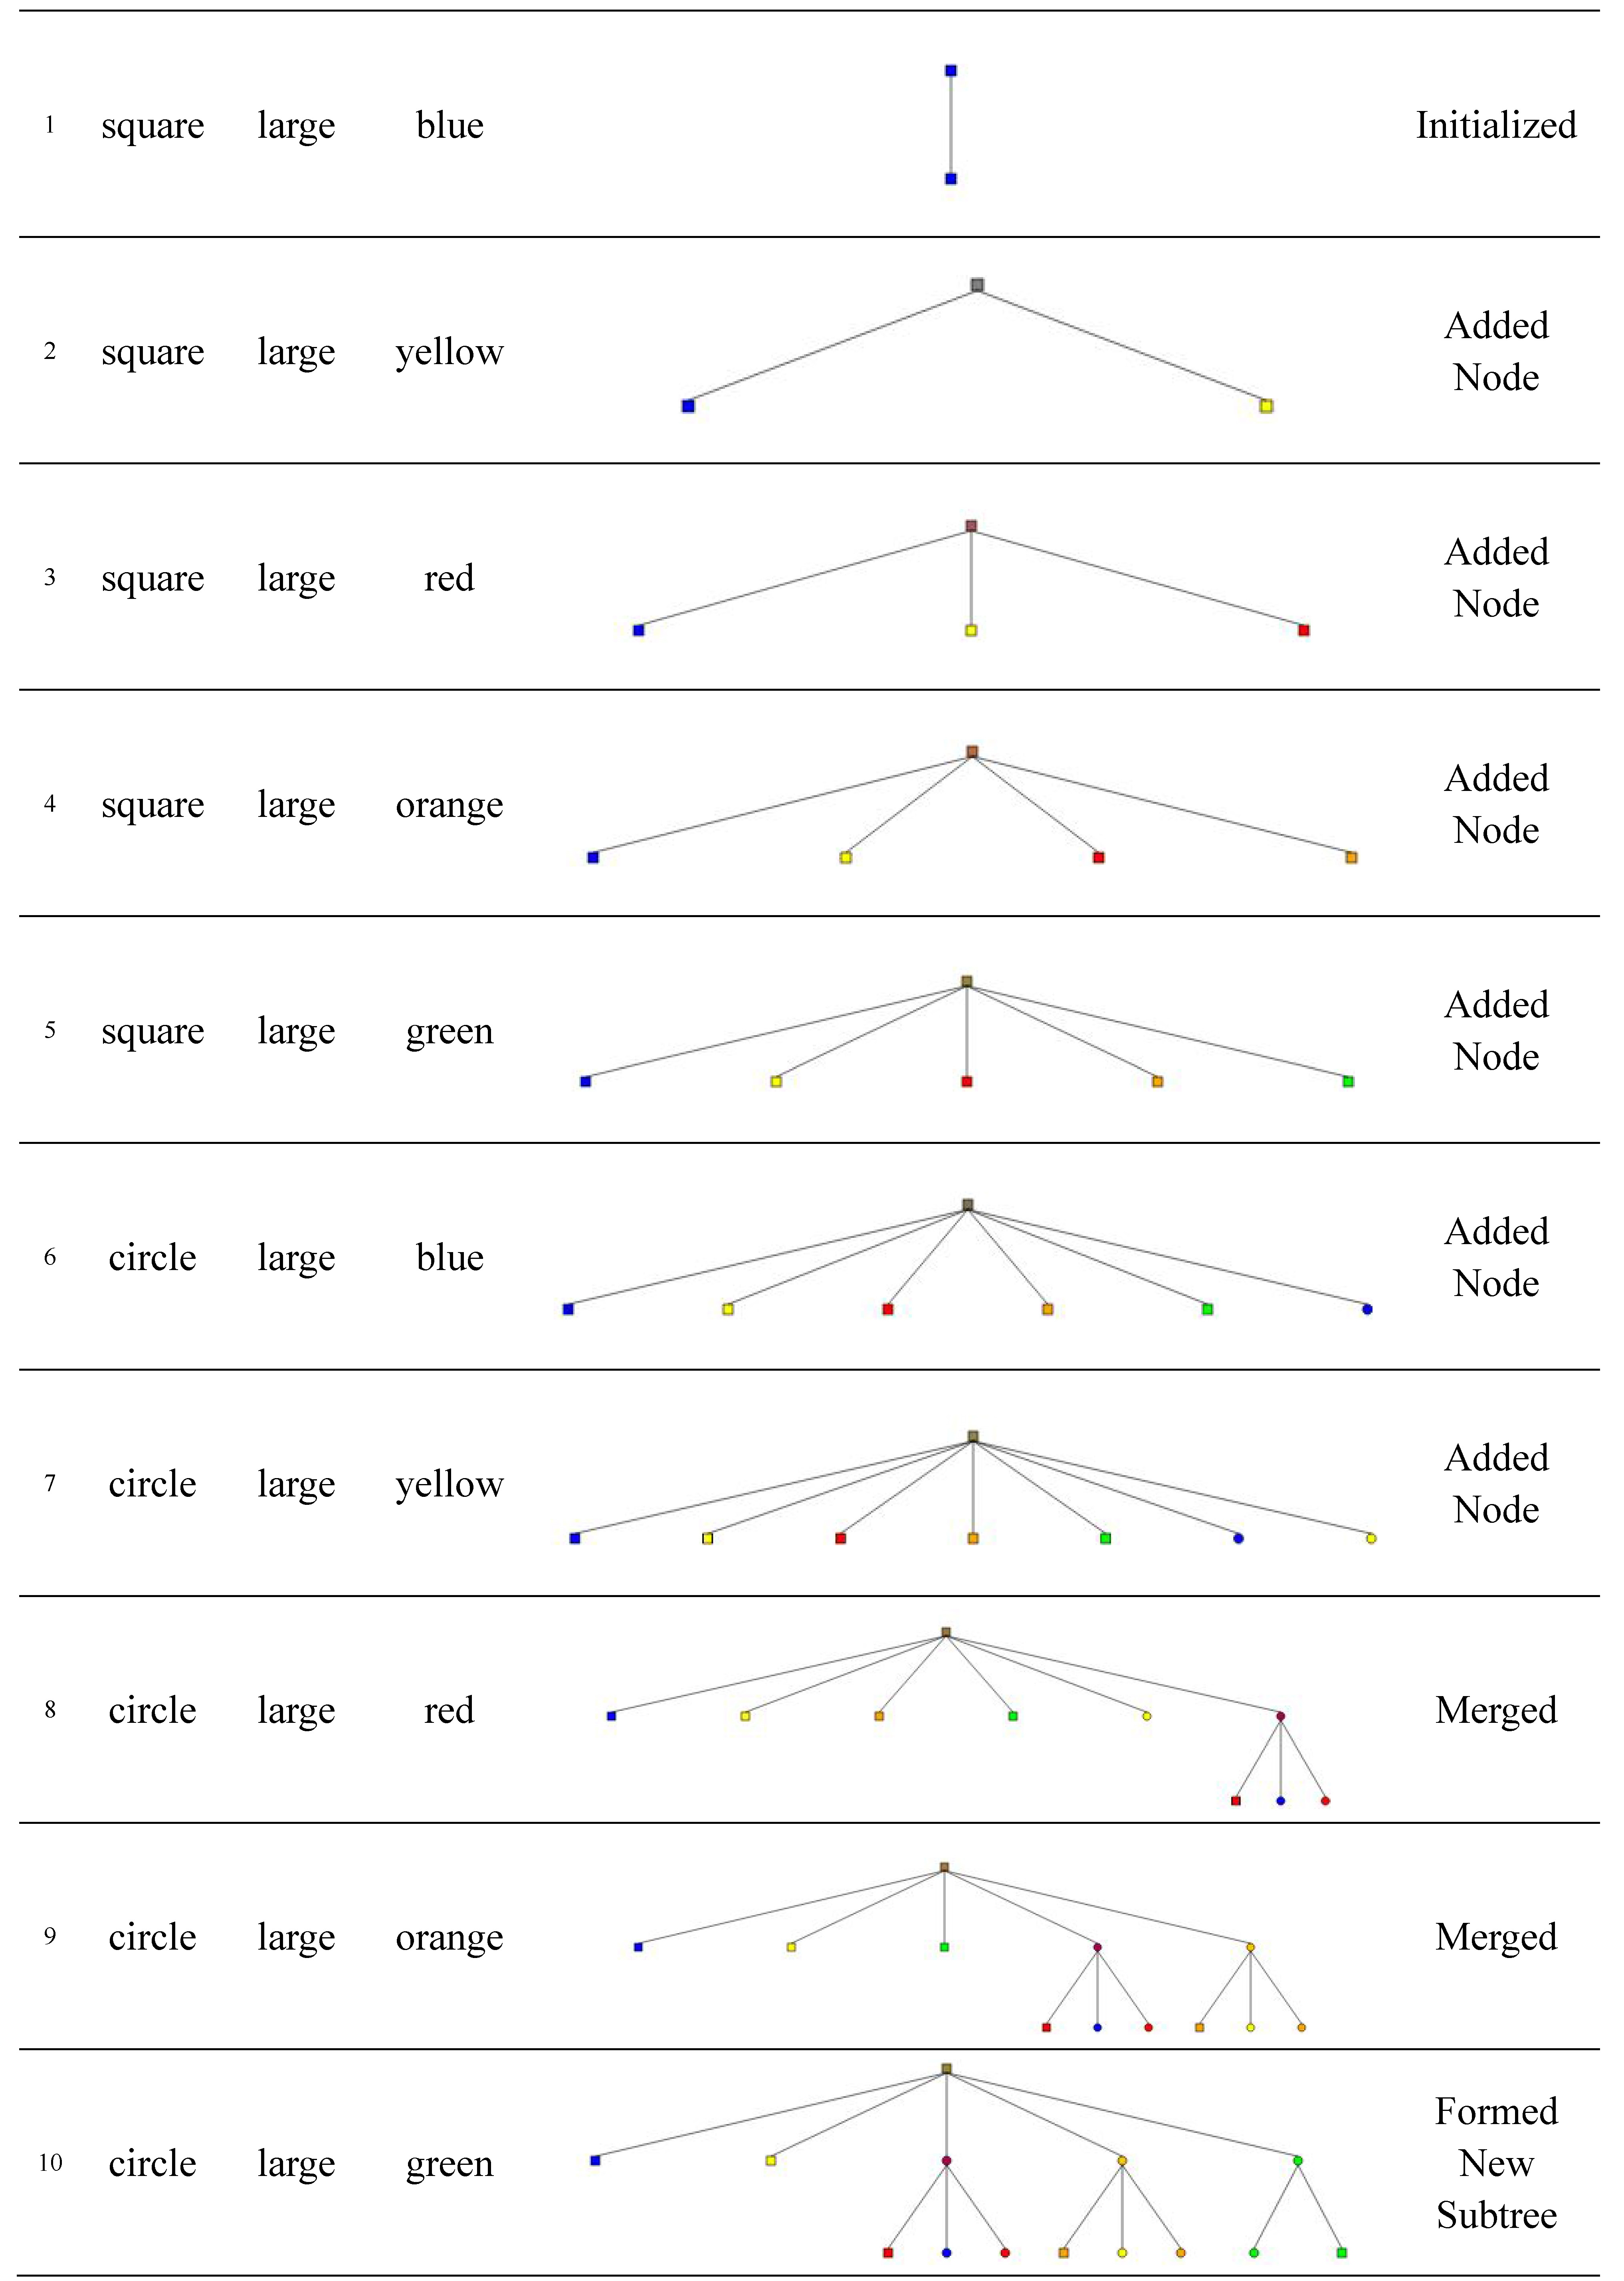
\includegraphics[width=420pt]{../images/inputseq1.jpg}
            \caption{The effect of input orders}
            \label{Fig:inputseq1}
 \end{figure}      

In the second experiment, we first input the blue square and blue circle and then followed by the yellow square and yellow circle and so on so forth till all the ten objects have been added. It's obvious that the tree is generated in a different way shown in the Figure\ref{Fig:inputseq2}.
\begin{figure}[h!]
            \centering
            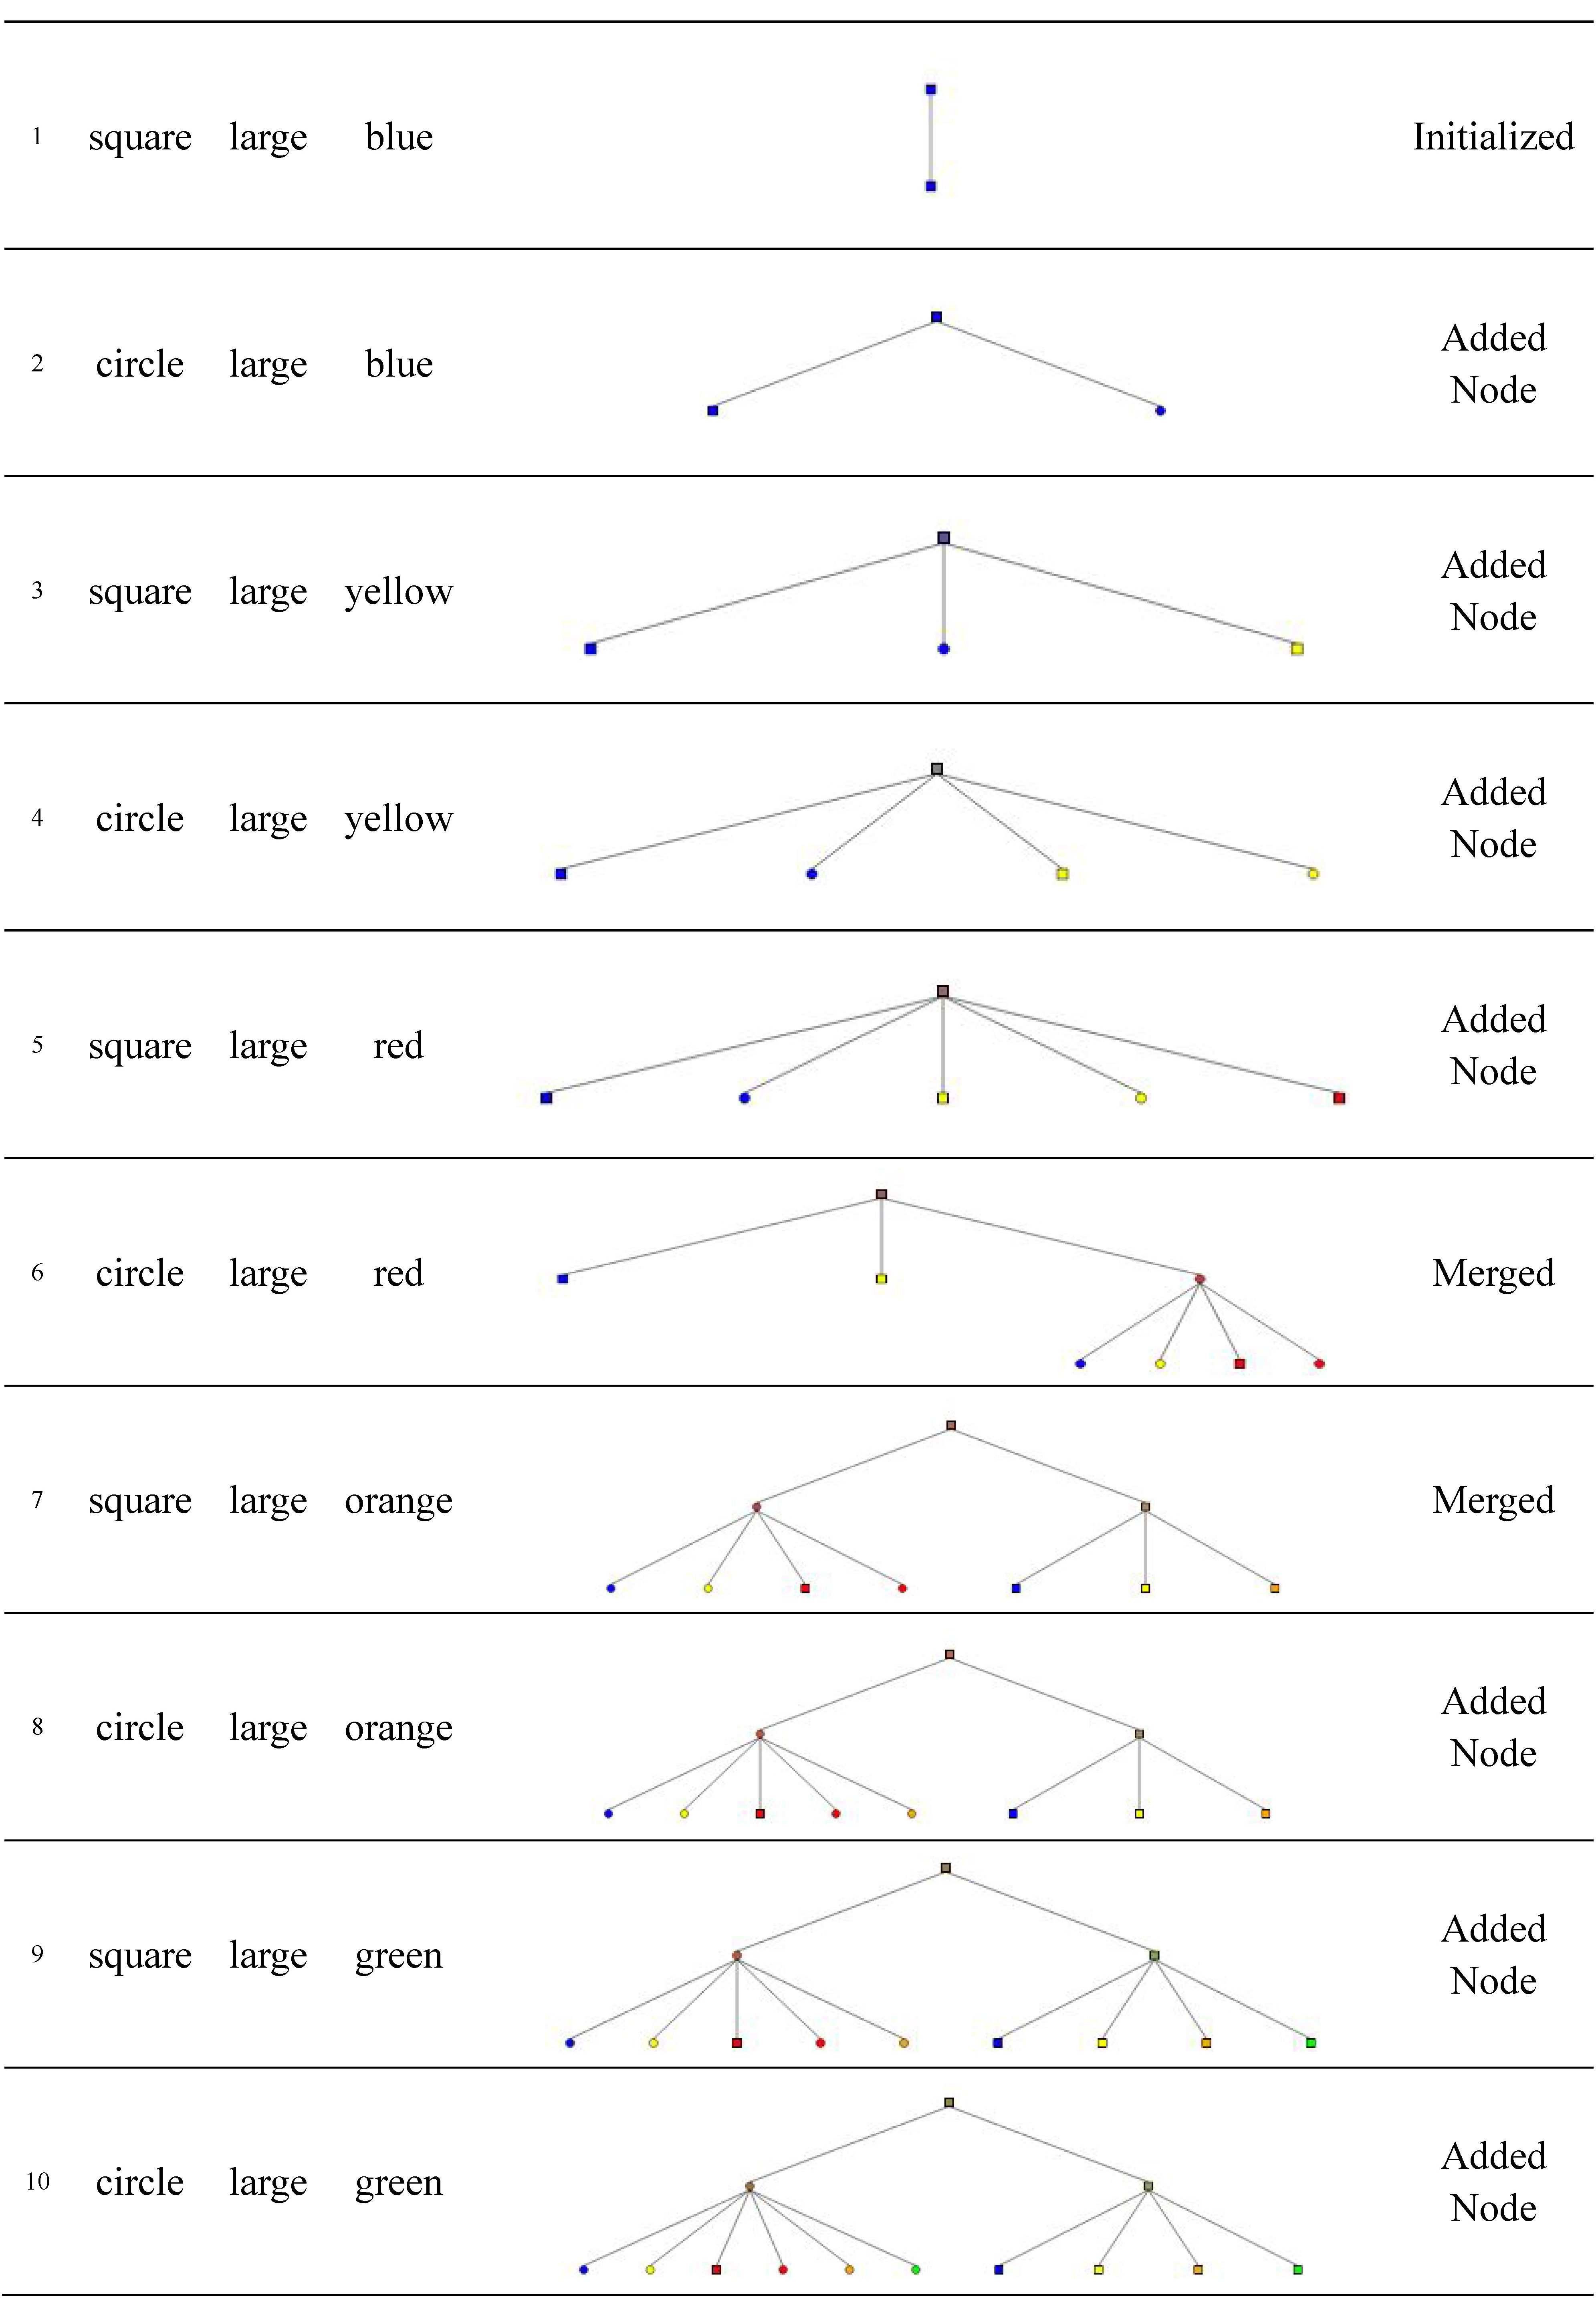
\includegraphics[width=420pt]{../images/inputseq2.jpg}
            \caption{The effect of input orders}
            \label{Fig:inputseq2}
 \end{figure}
 
 In the third experiment, we input the first three circles and then followed by the five squares and then the last two circles. The tree is generated in another way that is different from either of the previous two. The tree generated in the third experiment is shown in Figure\ref{Fig:inputseq3}.
 \begin{figure}[h!]
             \centering
             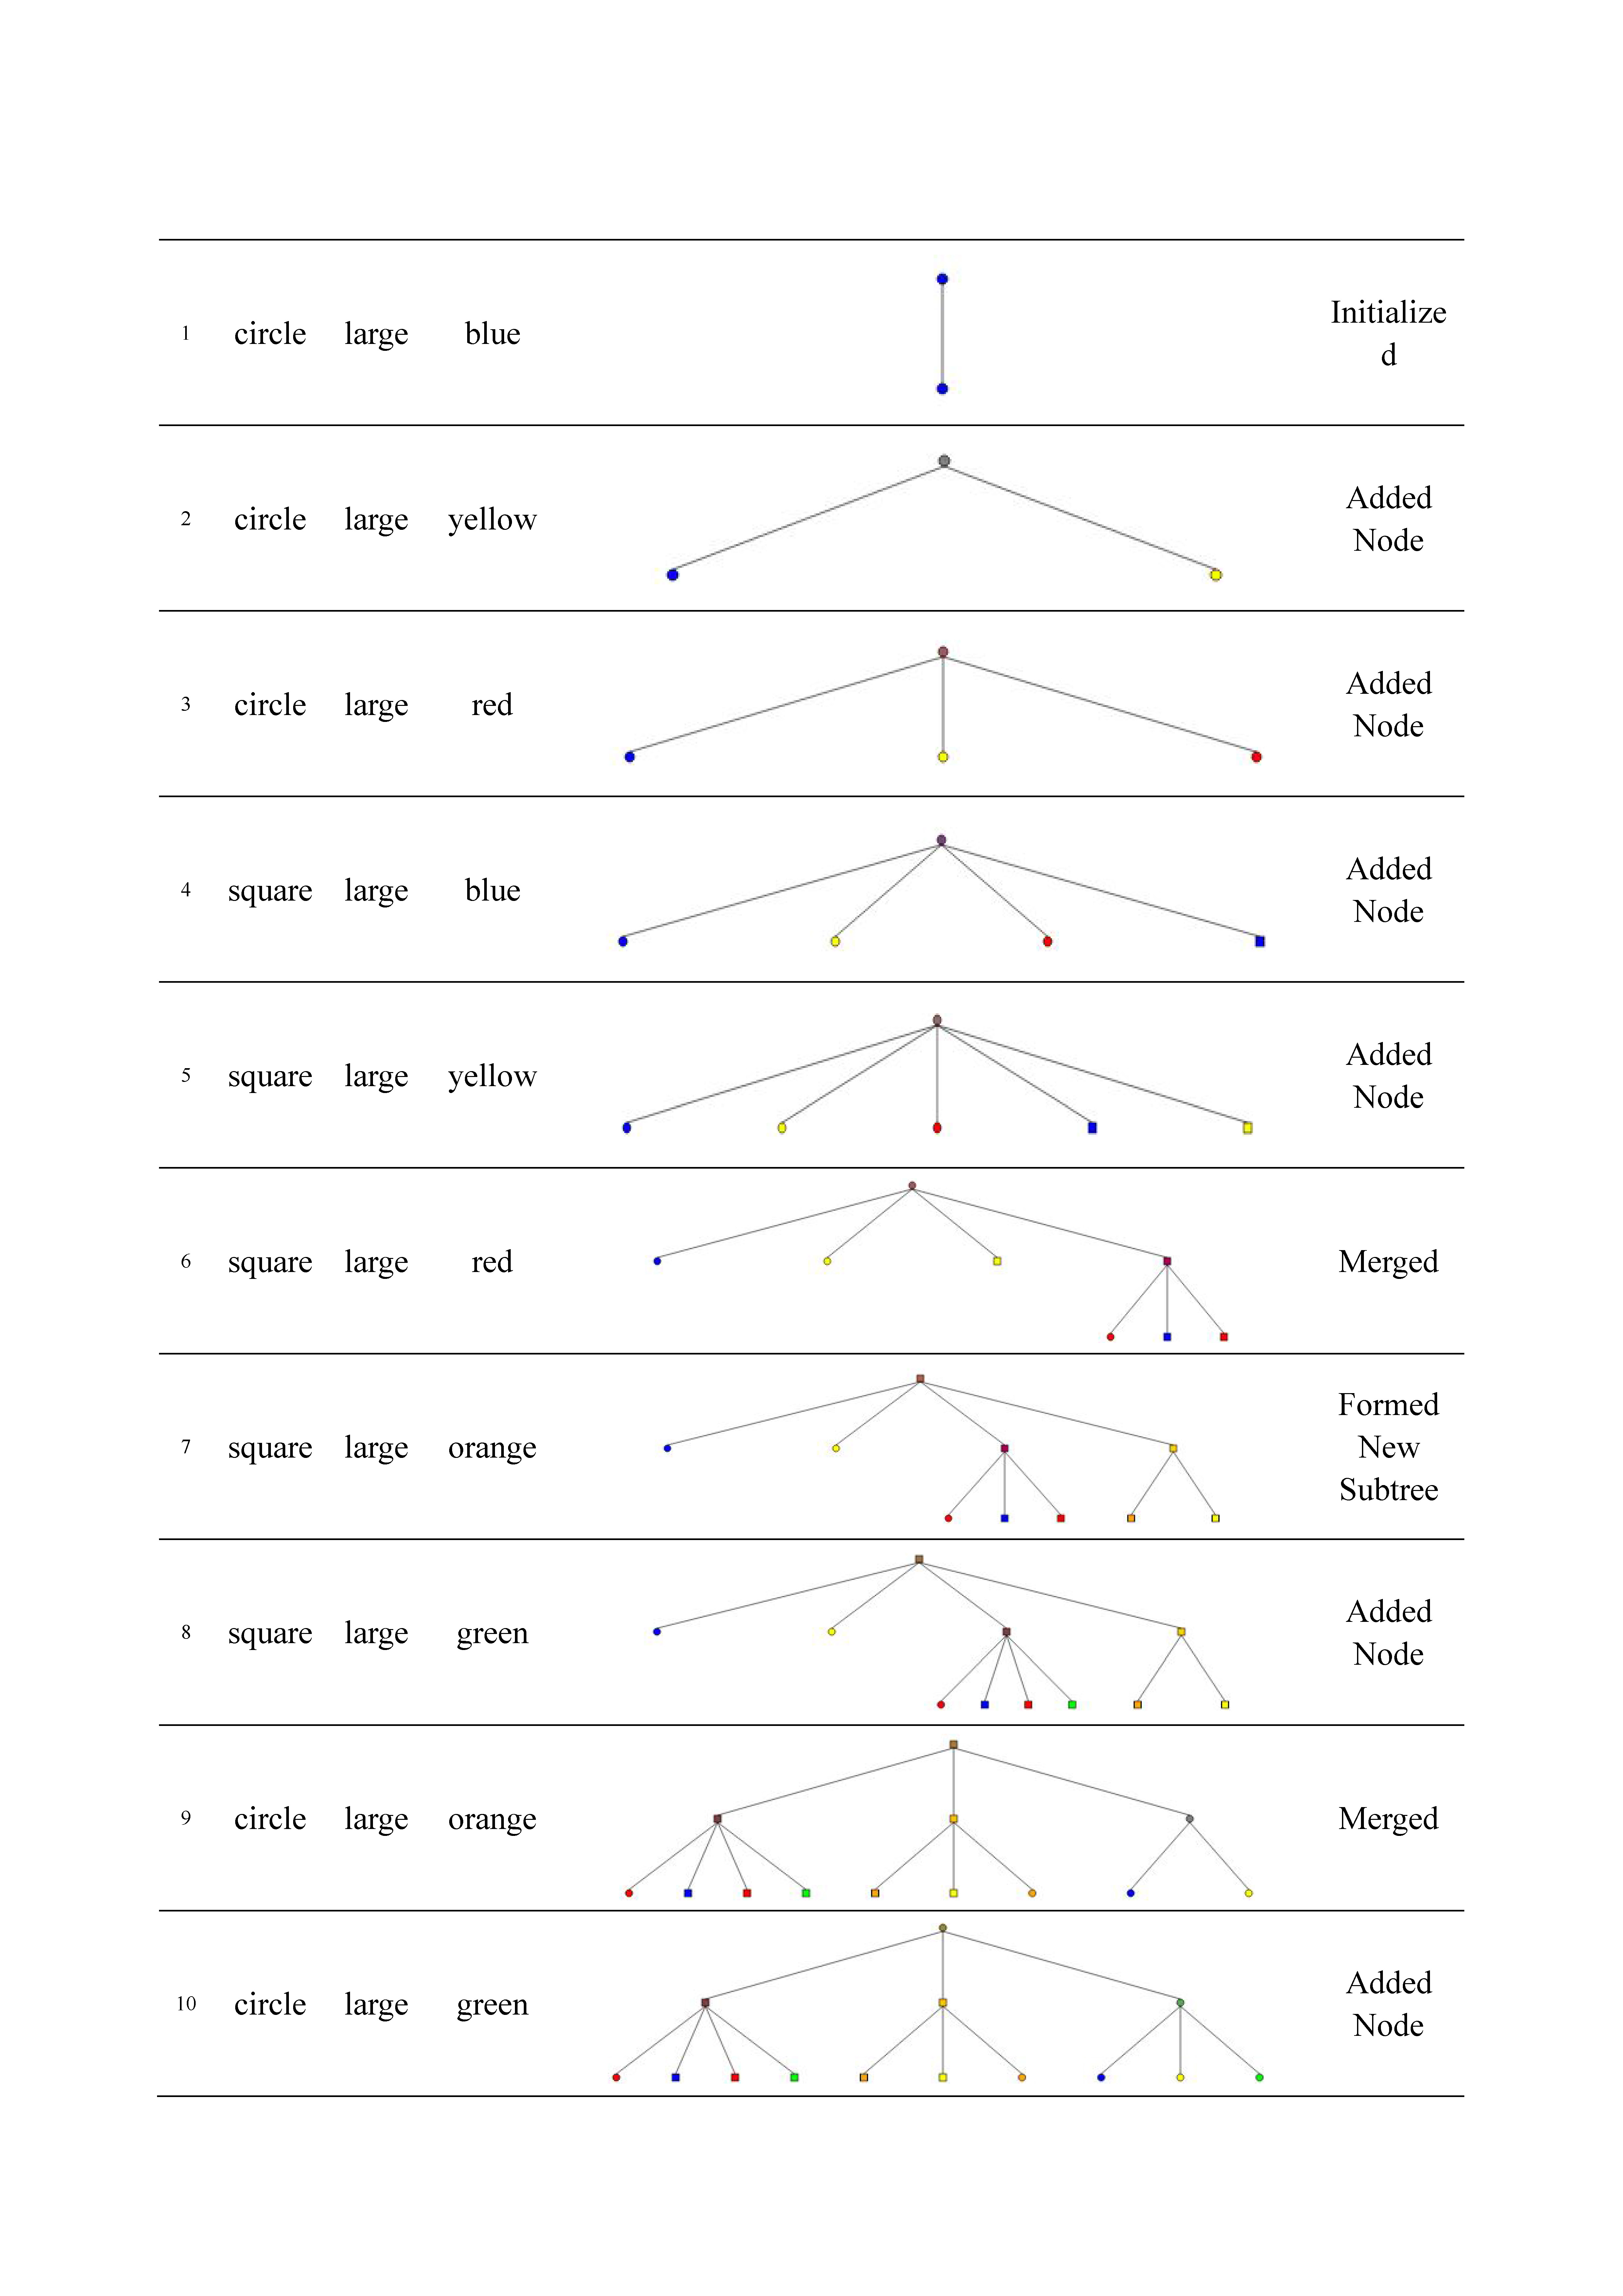
\includegraphics[width=420pt]{../images/inputseq3.jpg}
             \caption{The effect of input orders}
             \label{Fig:inputseq3}
  \end{figure}
 % %\newpage   
 %\includepdfmerge{../images/inputseq1.pdf}
 

    
    
    
%
% 4-dfsesign.tex
%
%  LaTeX source file for section  4 Design for the Conceptual Clustering lab module of the TAILS project.
%
\section{Design}
\subsection{The Interface}
Conceptual clustering module introduces COBWEB algorithm by presenting how a classification tree is generated based on user's input data. This simulation tool consists of two interfaces. The first one, corresponding to \lq\lq index.html\rq\rq, is for user to define or describe the objects that he wants to cluster, and the second one, corresponding to \lq\lq tree.html\rq\rq, is for user to input the defined object and observe the spanning of the classification tree. %The interface has three main components:

\subsection{The Class Diagram}
The class digram is shown in Figure \ref{Fig:ClassDiagram}. This diagram displays the variables and functions defined in each JavaScript file, the connections between each two files and the information transfered between them.
\begin{figure}[h!]
    \centering
    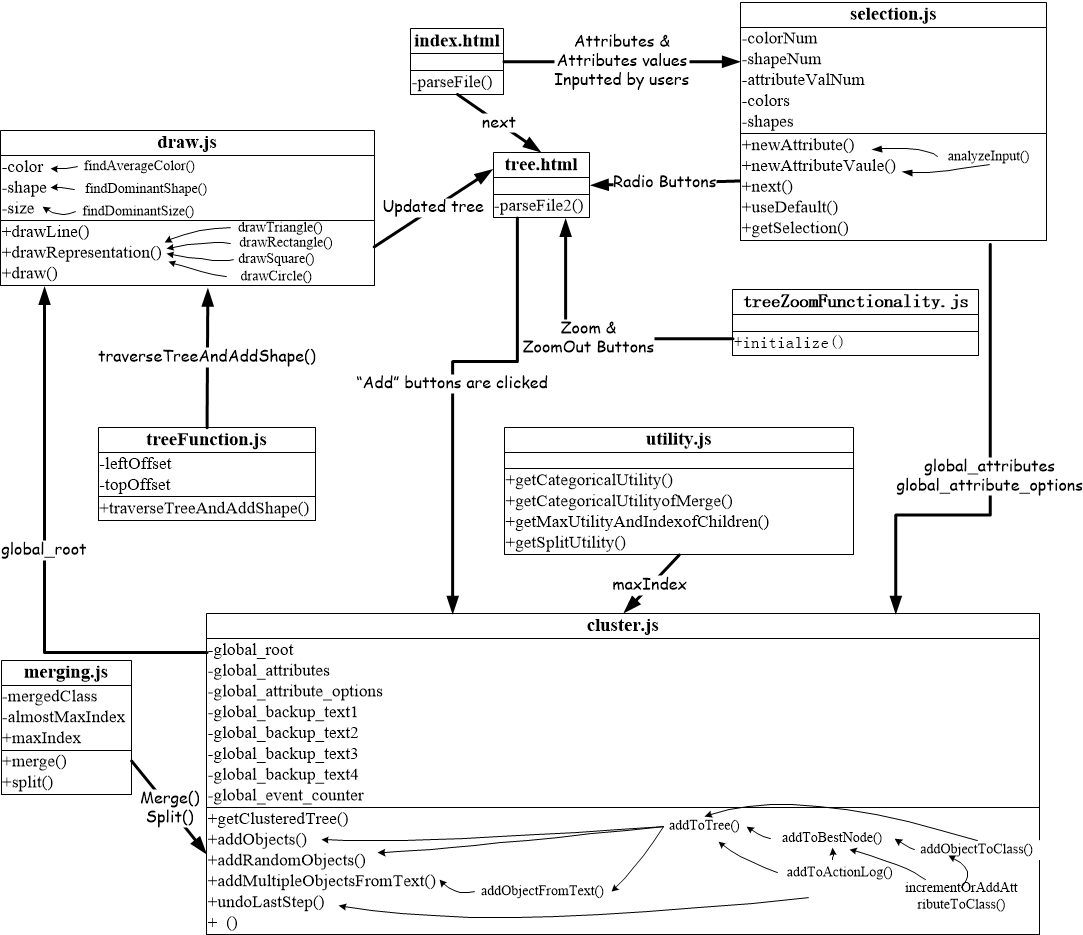
\includegraphics[width=400pt]{../images/class_diagram_for_Conceptual_Clustering.jpg}
    \caption{Class Diagram of TAILS Conceptual Clustering Module}
    \label{Fig:ClassDiagram}
\end{figure}

\subsection{The Sequence Diagram}
The sequence diagram is shown in Figure \ref{Fig:SequenceDigram}. It displays what actions from users can trigger which JavaScript file, the calling sequence of all the files and which function or variable is being transmitted between them.
\begin{figure}[h!]
    \centering
    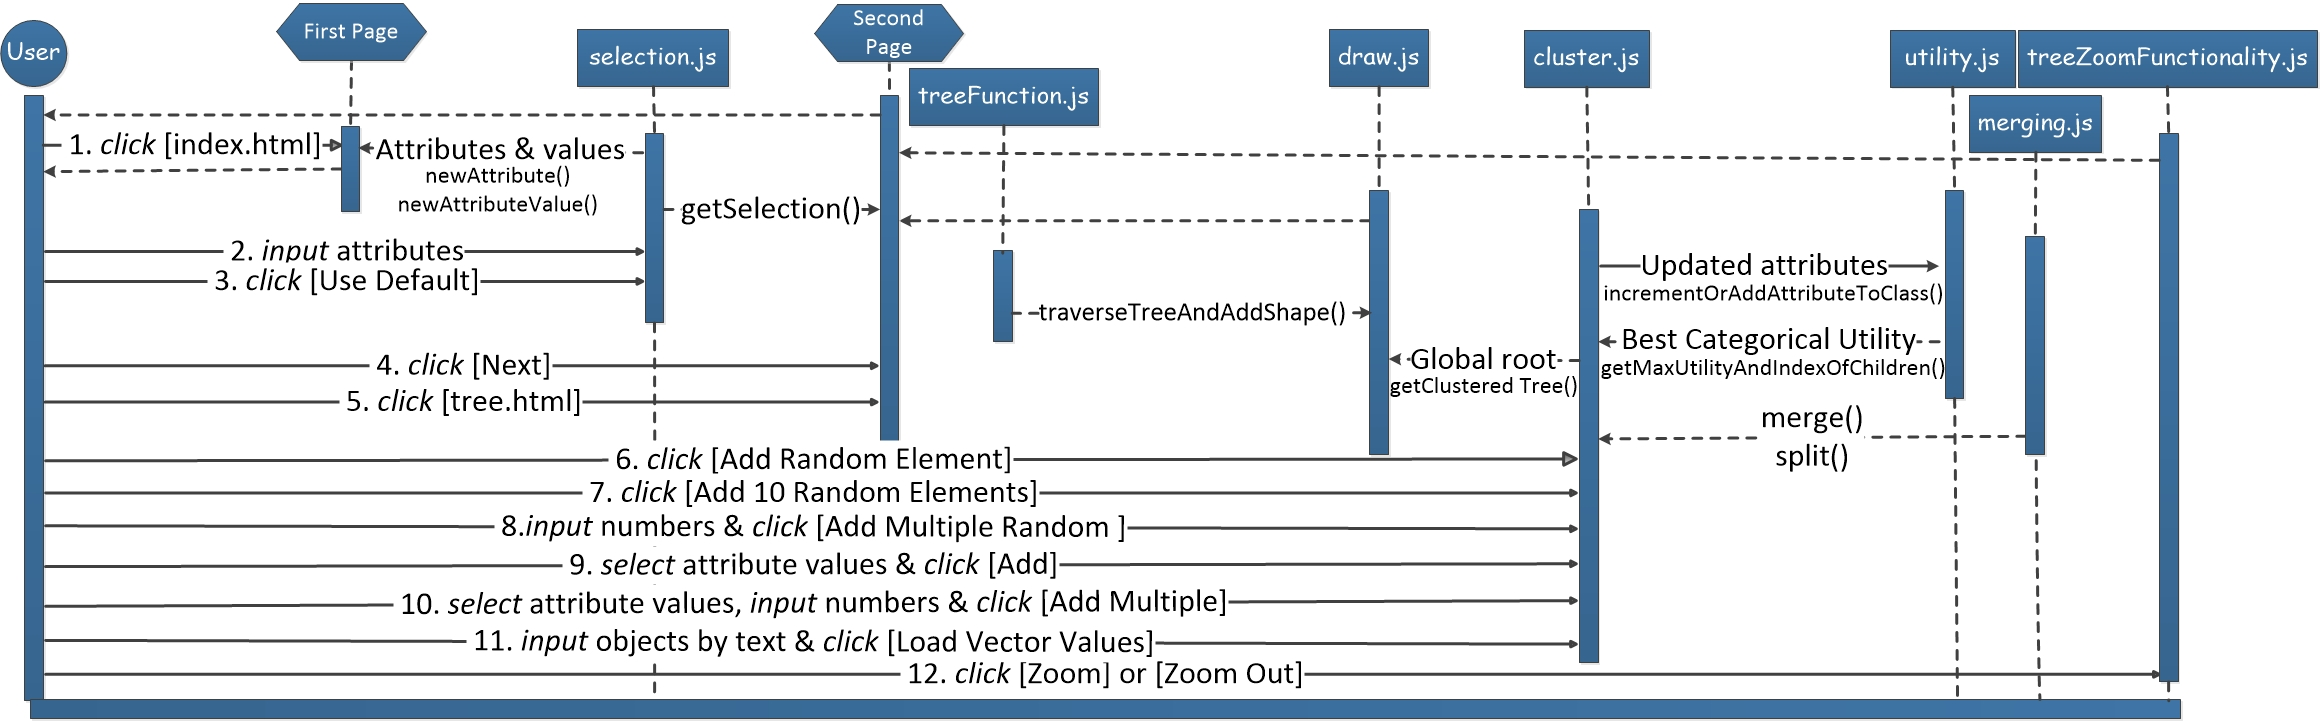
\includegraphics[width=400pt]{../images/sequence_diagram_for_Conceptual_clustering.jpg}
    \caption{Sequence Diagram of TAILS Conceptual Clustering Module}
    \label{Fig:SequenceDigram}
\end{figure}

\begin{comment}
\begin{itemize} \setlength{\itemsep}{0.01pt} %\itemsep-3pt
    \item Introduction,
    \item A user interface, and
    \item A classification tree visual.
\end{itemize}


\subsubsection{Introduction}
The introduction describes the use of the tool and explains the COBWEB algorithm. The description of the tool includes the instruction for custom input format and the procedures for inputting data. The explanation for the algorithm includes what specific operation is being carried out as a new object is added to the tree. The introduction not only shows how to use the simulation tool, but also relates the algorithm to the visual graphic tree generated by the algorithm, so that users can have a better understanding of how the COBWEB algorithm works.

\subsubsection{User Input}
Inputs for the conceptual clustering tool includes two parts: input for the attributes and attribute values and input for each object. There are three different ways for inputting attributes and values. System default supplies users with diverse attributes and various values. It's simple for users to get familiar with the COBWEB algorithm by the use of default attributes. Besides, the tool allows users to input their own data by the browser input or uploading a file. Either way, the attributes and values should be in the form of word only. No number or special characters are allowed. The other input is the object input by selecting specific attribute values defined by the first part. Adding one or multiple objects in fact generates a specific sequence for the input data. We have talked about the effect of the input orders for the tree generated in section 3.4. Users can also observe the effect by just playing the tool a little while.
\begin{itemize}\setlength{\itemsep}{0.01pt}
\item {Attributes and Attribute values}
\begin{itemize}\setlength{\itemsep}{0.01pt}
\item System default; 
\item Browser input;
\item And upload file of feature vectors.
\end{itemize}
\item {Input Sequence}
\end {itemize}
\subsubsection{Classification Tree Visual}
The classification tree will be generated while the object is being inputted. The user may either choose to add one object or multiple objects at a time.	The tool is able to generate tree for the selected objects or for random objects. For each node in the tree, there is a probabilistic concept label. Users can see the label by moving the mouse on the node. The label shows the conditional probability for each attribute value in the current cluster, which corresponds to $P(A_i=V_{ij}\left|C_k\right.)$, and the percentage of the current cluster against the whole tree which corresponds to $P(C_k)$.

\begin{figure}[h!]
    \centering
    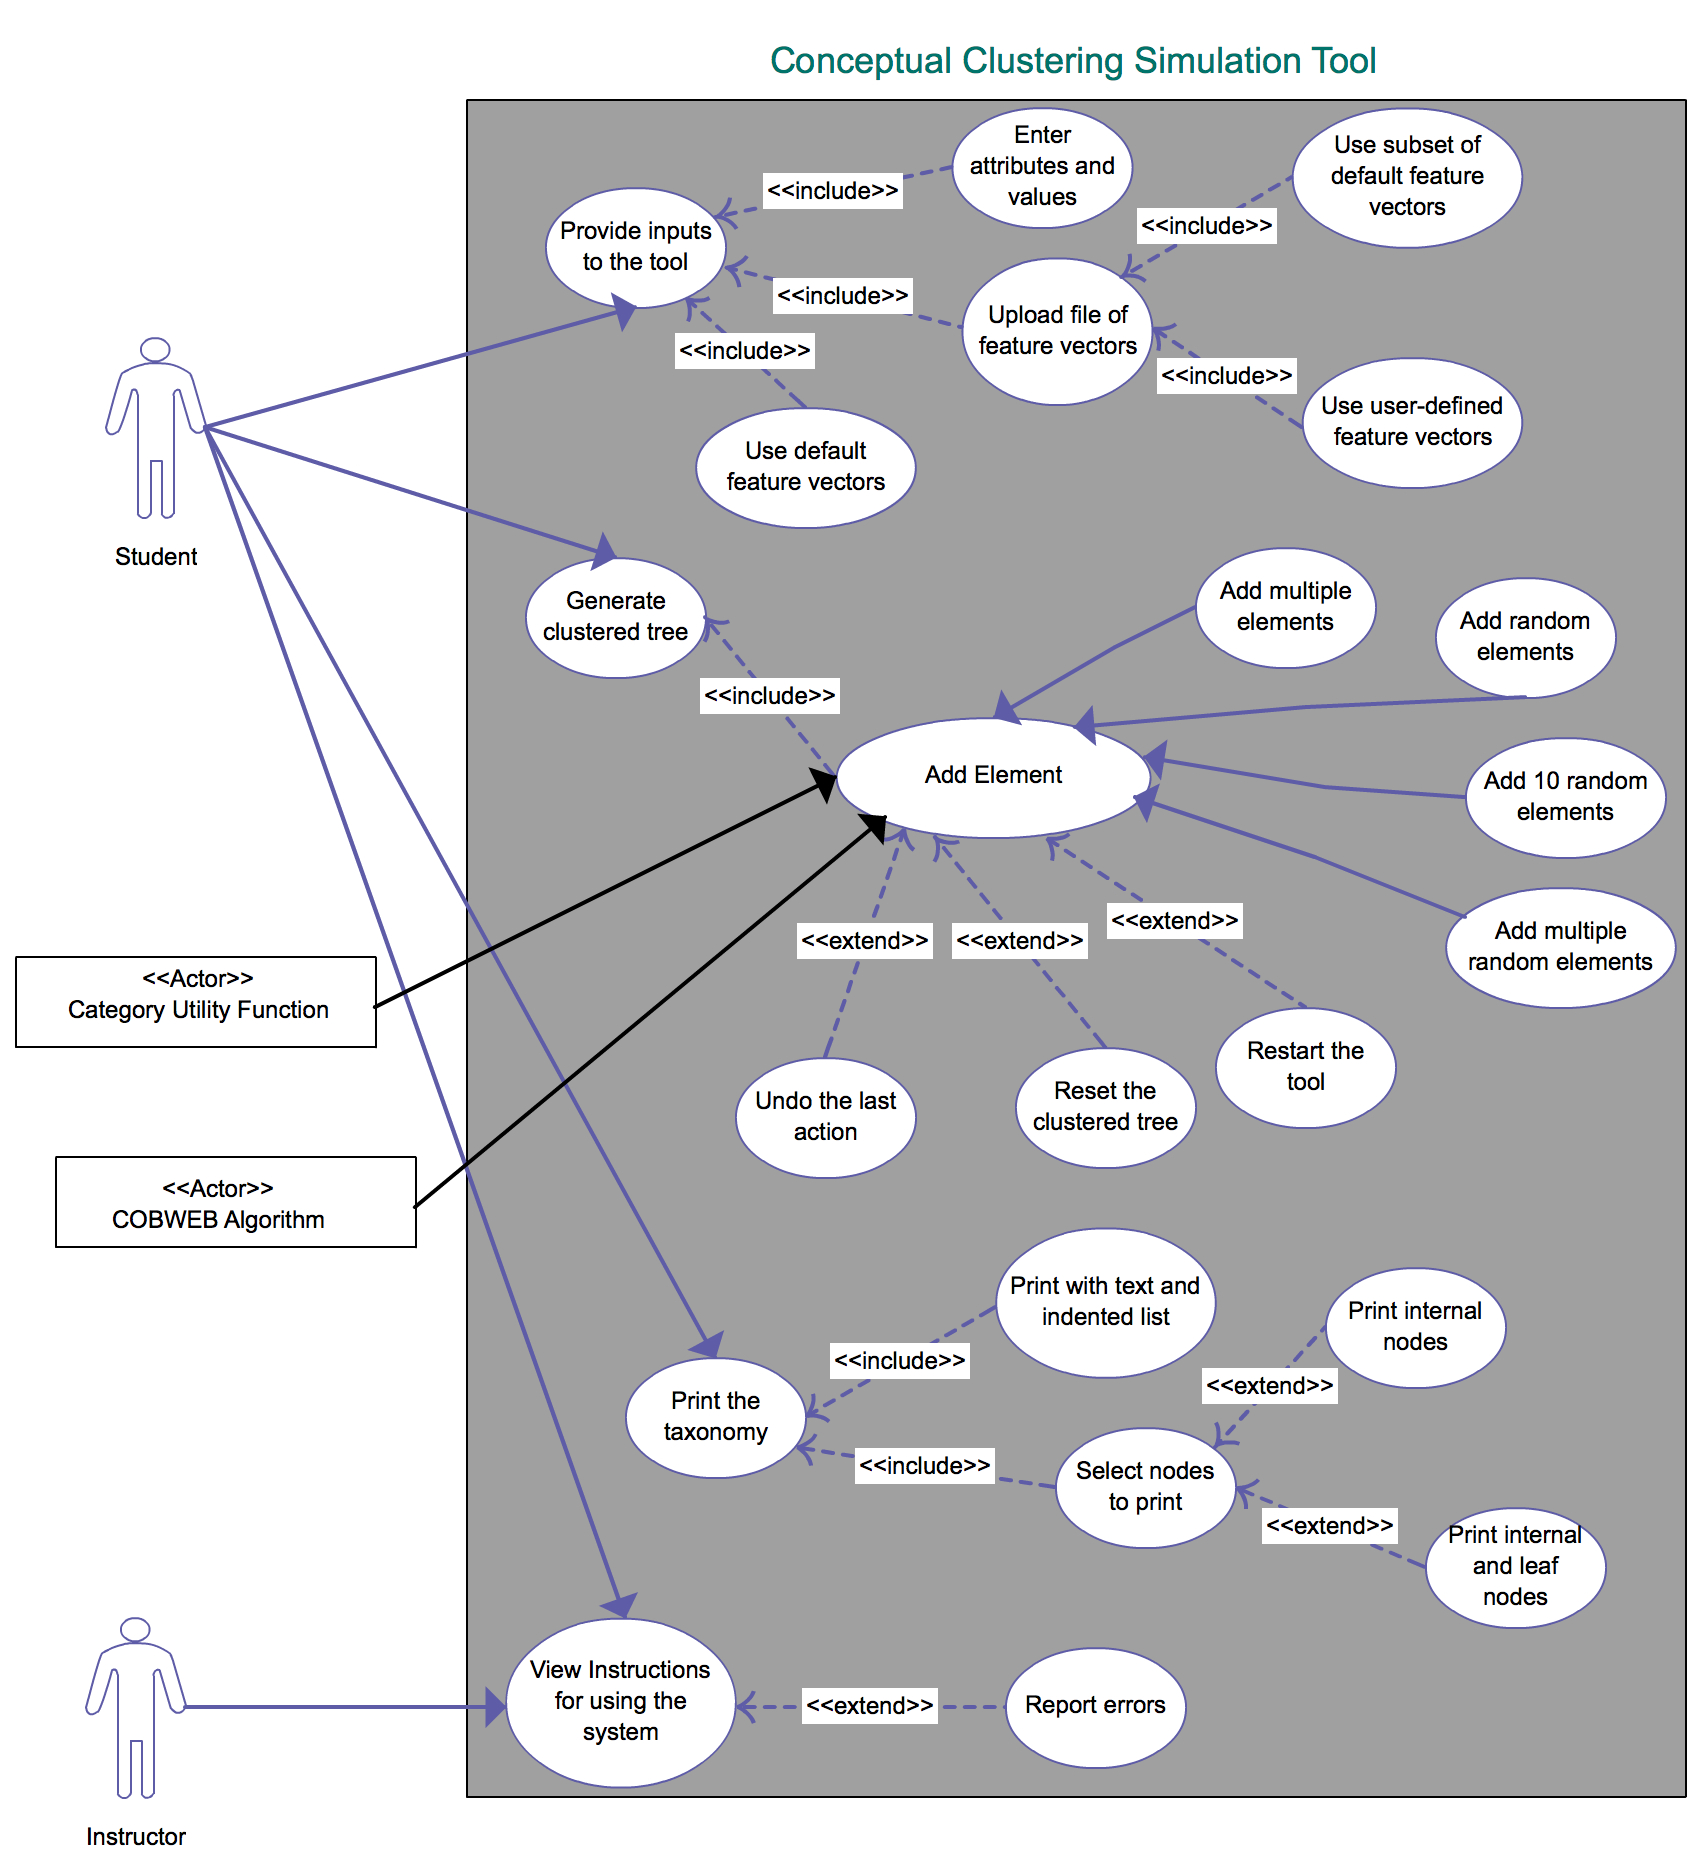
\includegraphics[width=400pt]{../images/Functional_CIM_Conceptual_Clustering.jpg}
    \caption{Use Case Diagram of TAILS Conceptual Clustering Module}
    \label{Fig:CIM}
\end{figure}

\end{comment}



% This module has the following requirements:

%\begin{enumerate}\itemsep-3pt
%\item There must be an introductory paragraph explaining what the module is and how to use it.
%\item The user must be able to select the start location.
%\item The user must be able to select the end location.
%\item The user must be able to select the search algorithm.
%\item The user must be able to run the program when they choose.
%\item The user must be able to see vertex names when the mouse hovers over any vertex.
%\item A graph visual portraying a search space must be created.
%\item A searchtree visual corresponding to the current actions of the search algorithm must be created.
%\end{enumerate}

%Requirement 1 requires a introductory text block on the webpage, requirements 2, 3, 4, and 5 correspond to user input which means the webpage
%must have a user interface component, requirement 6 will be a passive attribute of vertices, and requirements 7 and 8 will each be fulfilled by 
%providing the required visuals in subsections of the webpage.
%
%5-implementation-specific-HINTs.tex
%
%  LaTeX source file for section 5 Implementation Specific HINTs for the Conceptual Clustering lab module of the TAILS project.
%

\section{Implementation-Specific Design}

\subsection{The Code}
This program is built with JavaScript files: \emph{selection.js}, \emph{cluster.js}, \emph{utility.js}, \emph{merging.js}, \emph{draw.js}, \emph{treeFunction.js} and \emph{treeZoomFunctionality.js}. \emph{Cluster.js} is acting as the main script in the whole program. To aid with the implementation, the jQuery library and Raphael library are included as well.

\paragraph{index.html}:

This file forms the first interface and calls \emph{selection.js}.

\paragraph{selection.js}:

This script gets the attributes and attribute values if they are written in the right format. These attributes and values will be kept in the variable  \emph{global\_attributes} and \emph{global\_attribute\_options} defined in the function \emph{getSelection()} and will be used by \emph{cluster.js}.

Function \emph{getSelection()} also makes the radio buttons displayed in the second interface.

\paragraph{tree.html}:

This file forms the second interface and calls each of the JavaScript files for the clustering algorithm and presents a visual display of the classification tree. In the second interface, \emph{cluster.js} acts as the main function.


\paragraph{cluster.js}:

 A collection of functions which take in an object and add it to the tree in the proper location determined by a conceptual clustering algorithm. Once the object is added to the tree, the drawing is updated. \emph{cluster.js} is the script that implements the COBWEB algorithm.
 
 When the radio buttons are selected and \lq\lq{Add}\rq\rq or \lq\lq{Add Multiple}\rq\rq button is clicked, the program will go to the function \emph{addObject()}.
 
 When any of the three buttons that adds random object is clicked, the program will go to the function \emph{addRandomObject()}.
 
 When objects are inputted through the text and \lq\lq{Load Vector Values}\rq\rq button is clicked, the program will go to the function \emph{addMultipleObjectsFromText()}.
 
 When the \lq\lq{Undo Last Action}\rq\rq button is clicked, the program will go to the function \emph{undoLastStep()}.

All of the function \emph{addObject()}, \emph{addRandomObject()}, and \emph{addMultipleObjectsFromText()} calls the function \emph{addToTree()}.
 
\emph{addToTree()} calls \emph{addToBestNode()} if the tree is not empty; otherwise, it calls the function \emph{addObjectToClass()}.
 
\emph{addToBestNode()} is the function that implements the COBWEB algorithm. It finds the best place to put the new node in the tree depending on its categorical utility that is derived from the function \emph{getMaxUtilityAndIndexOfChildren()} in the file \emph{utility.js}. It also makes sure that if we're adding the object to a terminal node, to turn that node into a class with the two terminal nodes as its children. Once it is determined where the object should be placed, each attribute of the object is parsed through and added to the root node's attribute counts. It calls \emph{addObjectToClass()}.
 
Variable \emph{loopcheck} makes sure we're not in an infinite loop, that is trying to merge or split infinitely many times. Our stopping point for the infinite loop is trying to merge or split a full two cycles.

\emph{addObjectToClass()} physically adds the new object to its parent class and the attribute counts for that class are updated. It calls the function \emph{incrementOrAddAttributeToClass()}.
 
\emph{incrementOrAddAttributeToClass()} increments each attribute in the class by one. If the attribute doesn't exist in that class yet, it creates it.

\emph{getClusteredTree()} returns the handle on the root of the tree after the program executes the above functions and knows where to put the new object. \emph{getClusteredTree()} will be used by the function \emph{draw()} in the file \emph{draw.js}.

\paragraph{utility.js}:

This script generates the categorical utility of adding a new object to the tree in relation to a specific node. The equation it uses to generate the categorical utility is show in Page 5.

\emph{getMaxUtilityAndIndexOfChildren()} acts as the main function in the \emph{utility.js}. It creates an object that contains the two classes with the best categorical utilities. Then it decides if it is best to put the new object in an already existing class, merge two classes, or to make it its own class. It transmits the variable \emph{maxIndex} and \emph{maxUtil(utility)} to the function \emph{addToBestNode()} in the file \emph{cluster.js}. It calls \emph{getCategoricalUtility()} and \emph{getCategoricalUtilityOfMerge()}. 
 
\emph{getCategoricalUtility()} finds the expected number of attribute values that can be correctly guessed and adds this number to the predicted number of correctly guessed attribute values that already exist. \emph{getExpectedNumberOfAttributeToGuess()} is called.

\emph{getCategoricalUtilityOfMerge()} returns the categorical utility if the algorithm were to decide to merge the two classes with the highest categorical utilities. It calls \emph{getExpectedGuessForMergedClasses()}.

\emph{getExpectedGuessForMergedClasses()} temporarily adds the object to the hypothetically merged classes to compute the categorical utility of placing the object in this merged class.

\emph{getExpectedNumberOfAttributeToGuess()} returns the number of expected attributes  that would be correctly guessed for the class that is passed in.

\emph{getSplitUtility()} calculates the categorical utility of splitting an already existing class into separate classes.

\paragraph{merging.js}:

\emph{merge()} takes the two objects/classes with the best categorical utility and first checks to see if they have children. If both of them are just terminal nodes, then it parses through their attributes and adds them to a parent node which will now be their parent class. Then it adds the new object to this merged class. If one of them is a class, then it just adds the attributes of the other best object to the class. If they're both classes, it takes all of the children of one class and adds them as children to the other class.

\emph{split()} adds all of the children of a class to the level the parent is at in the tree and then removes the parent class from the tree.

\paragraph{draw.js}:

\emph{draw()} acts as the main function in \emph{draw.js}. It clears the paper if anything is there, then creates the raphael object and draws the tree. \emph{draw()} gets the updated tree from the function \emph{getClusteredTree()} in the \emph{cluster.js} file. It calls the function \emph{traverseTreeAndAddShape()} in the file \emph{treeFunction.js} which takes in a tree and traverses that tree from the root down.

\emph{drawShape()} and \emph{drawLine()} are acting as the sub-main functions in file \emph{draw.js}. \emph{drawShape()} calls \emph{findAverageColor()}, \emph{findDominantShape()}, \emph{findDominantSize()} and \emph{drawRepresenataion()}. 

\emph{drawLine()} creates a line between the new node and its parent node.

\emph{drawRepresenataion} calls  \emph{drawCircle()}, \emph{drawRectangle()},  \emph{drawTriangle()} and  \emph{drawSquare()}. These four functions create a corresponding shape at a specific spot on the canvas.
    
\paragraph{treeFunctions.js}:

\emph{traverseTreeAndAddShape()} first checks if the root node exists, if it doesn't then it creates the root node as well as the canvas on which the tree will exist. If the root node exists, it finds the placement of each of the child objects of the root node as well as drawing a line between each object and its parent node. 

\paragraph{treeZoomFunctionality.js}:

This script fulfills the zoom function in the second interface.
    
\subsection{COBWEB Algorithm}
    The COBWEB Algorithm is:
    \begin{itemize}\itemsep-3pt
    \item 
    Cobweb( Node, Instance)\\
    begin\\
    \item if Node is a leaf then begin\\
    		\begin{itemize}\itemsep-3pt
           	\item create two children of Node, L1 and L2;\\
           	\item set the probabilities of L1 to those of Node;\\
          	\item initialize the probabilities for L2 to those of instance;\\
           	\item add instance of Node, updating Node’s probabilities;\\
            end;
            \end{itemize}
    \item  else if Node is not a leaf\\   
      add Instance to Node, updating Node’s probabilities;
      for each child, C, of Node, compute the category utility of the clustering achieved by placing instance in C;   
      \begin{itemize}\itemsep-3pt
      \item let S1 be the score for the best categorization, C1;\\
      \item let S2 be the score for the second best categorization, C2;\\
      \item let S3 be the score for placing instance in a new category;\\
      \item let S4 be the score for merging C1 and C2 into one category;\\
      \item let S5 be the score for splitting C1(replacing it with its child categories)\\
      end;
      \end{itemize}
      
    \item if S1 is the best score, then cobweb(C1, Instance)\\
    \item else if S3 is the best score, then initialize the new category’s probabilities to those of instance\\
    \item else if S4 is the best score, then cobweb (Cm, Instance), where Cm is the result of merging C1 and C2;\\
    \item  else if S5 is the best score, then split C1; cobweb(Node, Instance)\\
    end;
    \end{itemize}
%
%6-test-suite-and-drivers.tex
%
%  LaTeX source file for section 6 Test Suite and Drivers for the Conceptual Clustering lab module of the TAILS project.
%
\section{Test Suite and Drivers}

\subsection{Using the default setting}
Click \emph{Use Default} in the first interface and then follow these five steps. 
\begin{enumerate}[1)]
\item Choose \emph{circle,large,green}, enter \emph{8} in the \emph{Add Multiple} button and click it.
\item Choose \emph{circle,large,red}, enter \emph{2} in the \emph{Add Multiple} button and click it.
\item Choose \emph{square,small,green}, enter \emph{4} in the \emph{Add Multiple} button and click it.
\item Choose \emph{square,small,blue}, enter \emph{7} in the \emph{Add Multiple} button and click it.
\item Choose \emph{circle,large,blue} and click the \emph{Add} button.
\end{enumerate}

Or you may choose \emph{Use Default} in the first interface and then load the following text to the text box at the bottom of the second interface.\\
circle,large,green!circle,large,green!circle,large,green!circle,large,green!circle,large,green!\\circle,large,green!circle,large,green!circle,large,green!circle,large,red!circle,large,red!\\square,small,green!square,small,green!square,small,green!square,small,green!square,small,blue!\\square,small,blue!square,small,blue!square,small,blue!square,small,blue!square,small,blue!\\square,small,blue!circle,large,blue!

Either way, a classification tree shown in Figure\ref{Fig:testsuite} will be generated. We can see that the last object, a blue circle is grouped to the class consists of two red circles and eight green circles. The remaining objects, including four green squares and seven blue squares are in the same class. This classification tree corresponds to the example on Page 5. 
\begin{figure}[h!]
    \centering
    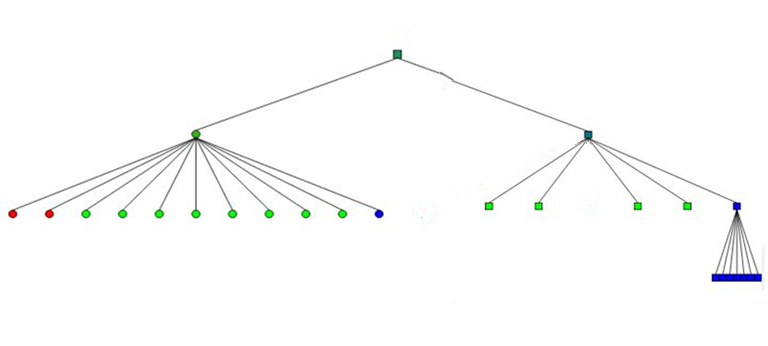
\includegraphics[width=300pt]{../images/testsuite.jpg}
    \caption{}
    \label{Fig:testsuite}
	\end{figure}
%
%7-experiments.tex
%
%  LaTeX source file for section 7 Experiments for the Conceptual Clustering lab module of the TAILS project.

\section{Experiments}
The purpose of this section is to introduce students to the conceptual clustering simulation tool, clustering algorithms, feature vectors, probability, and the effect of input ordering on the learning that takes place when an application is trained on a set of data. Students with an understanding of Bayes Theorem will be able to study the category utility function used to rank the potential clusters each time a training vector is added to the set.

\subsection{Experiment 1}
\paragraph{Observe the effect of input ordering on COBWEB}
The first exercise provides students the opportunity to observe first-hand effect of input ordering on the taxonomy constructed by the COBWEB conceptual clustering algorithm\cite{fisher1987knowledge,fisher1995optimization,gennari1989models}. 
\subparagraph{Objective} 
This exercise demonstrates via experimentation the value of random ordering of input to a learning algorithm. Students use an implementation of the COBWEB conceptual clustering algorithm to visualize the taxonomy of clusters created for a set of feature vectors given as input. The internal or summary nodes of the resulting tree are displayed as objects that reflect the average color and size of the objects in the subtree rooted at the node and the most frequently occurring shape in the subtree.
\subparagraph{Experiment Description} Start the Conceptual Clustering simulation tool and use the default attributes. Then input the following objects one by one in the order shown in Table \ref{tab:exp1seq1} and Table \ref{tab:exp1seq2} and observe the way the tree generated. Understand the concept label of parent nodes in each tree.

\begin{table}[!ht]
 \ttabbox{\caption{Experiment1: Input Sequence 1}}
 {
 \centering
 \begin{tabular}{l l l l l l l l}\hline
 \textbf{} & \textbf{shape} & \textbf{size} & \textbf{color}   & \textbf{} & \textbf{shape} & \textbf{size} & \textbf{color}\\\hline
 \textbf{1} & \textbf{square} & \textbf{large} & \textbf{blue}   & \textbf{6} & \textbf{circle} & \textbf{large} & \textbf{blue}\\
 \textbf{2} & \textbf{square} & \textbf{large} & \textbf{yellow} & \textbf{7} & \textbf{circle} & \textbf{large} & \textbf{yellow}\\
 \textbf{3} & \textbf{square} & \textbf{large} & \textbf{red}    & \textbf{8} & \textbf{circle} & \textbf{large} & \textbf{red}\\
 \textbf{4} & \textbf{square} & \textbf{large} & \textbf{orange} & \textbf{9} & \textbf{circle} & \textbf{large} & \textbf{orange}\\
 \textbf{5} & \textbf{square} & \textbf{large} & \textbf{green}  & \textbf{10} & \textbf{circle} & \textbf{large} & \textbf{green}\\
 \hline
 \end{tabular}
 \label{tab:exp1seq1}}
 \end{table}
 
\begin{table}[!ht]
 \ttabbox{\caption{Experiment 1: Input Sequence 2}}
 {
 \centering
 \begin{tabular}{l l l l l l l l}\hline
 \textbf{} & \textbf{shape} & \textbf{size} & \textbf{color}   & \textbf{} & \textbf{shape} & \textbf{size} & \textbf{color}\\\hline
 \textbf{1} & \textbf{square} & \textbf{large} & \textbf{blue}   & \textbf{6}& \textbf{circle} & \textbf{large} & \textbf{red}\\
 \textbf{2} & \textbf{circle} & \textbf{large} & \textbf{blue}   & \textbf{7}& \textbf{square} & \textbf{large} & \textbf{orange} \\
 \textbf{3} & \textbf{square} & \textbf{large} & \textbf{yellow} & \textbf{8}& \textbf{circle} & \textbf{large} & \textbf{orange} \\
 \textbf{4} & \textbf{circle} & \textbf{large} & \textbf{yellow} & \textbf{9}& \textbf{square} & \textbf{large} & \textbf{green} \\
 \textbf{5} &\textbf{square} & \textbf{large}  & \textbf{red}    &\textbf{10}& \textbf{circle} & \textbf{large} & \textbf{green}\\
 \hline
 \end{tabular}
 \label{tab:exp1seq2}}
 \end{table}
 
 \subsection{Experiment 2}
 \paragraph{Think of any possible application of conceptual clustering algorithm COBWEB in real life} This exercise provides students the opportunity to think seriously about COBWEB algorithm and understand relevant concepts. 
 \subparagraph{Objective} Experiment 2 allows students to demonstrate a deep understanding of the conceptual clustering algorithm COBWEB by describing an example in details. Students are expected to be able to tell a clustering problem from a classification problem, and understands concepts of attribute and attribute values by representing objects in their example using feature vectors.
 \subparagraph{Experiment Description} Think of any possible application of conceptual clustering algorithm COBWEB in our life. Try to describe your example in the following aspects: 1)Why it is a clustering problem instead of a classification problem; 2)What might be the \emph{concept label} for a cluster in your example; 3)What might happen when a new item is added in your example, referring to the four operations of COBWEB.
 
 Then try to write down some possible attributes and attribute values of your example and keep it in a text file. Load your attributes and values through the text box in the first interface. Be sure that the attribute should be recorded in the first line and ended with a \lq\lq{\#}\rq\rq. The next line will be the values for the first attribute and so on so forth. The attributes and attribute values of a possible example about one kind of machines are shown here.\\
 \emph{type,rate,weight,pricerange\#\\
 modelbased,conceptbased,experiencebased\#\\
 excellent,good,average,unknown\#\\
 heavy,light\#\\
 high,low\#\\
 verysmall,small,medium,large,extralarge\#\\}
 
Last, try to write down one possible order for the items in your example and keep it in a text file. Load your sequence of those items through the text box in the second interface. Be sure that each item should be ended with a \lq\lq{!}\rq\rq. A possible input sequence for the example above is shown below:\\
\emph{modelbased,excellent,light,high,verysmall!\\
modelbased,good,light,high,verysmall!\\
modelbased,unknow,heavy,low,medium!\\
conceptbased,average,heavy,low,large!\\
conceptbased,average,heavy,high,verysmall!\\
conceptbased,excellent,heavy,high,verysmall!\\
experiencebased,good,light,low,medium!\\
experiencebased,unknown,light,high,small!\\}
 
 \subsection{Experiment 3}
 \paragraph{Calculate the Category Utility for the following example} This exercise is designed for those students who have a basic knowledge of probability, conditional probability and Bayes Theorem. 
 \subparagraph{Objective} This exercise demonstrates the ability to understand the evaluation function Category Utility in COBWEB algorithm. Students are expected to have a better idea of Category Utility by doing the calculations. 
 \subparagraph{Experiment Description} There are two classes, denoted as $C_1$ and $C_2$. Objects contained in $C_1$ and $C_2$ are shown in Table\ref{tab:experiment2}. There are three attributes \emph{color}, \emph{shape} and \emph{size} with seven attribute values which are: $A_1=\{\text{color}|V_{11}=\text{Green},V_{12}=\text{Red}, V_{13}=\text{Blue}\}$
 $A_2=\{\text{shape}|V_{21}=\text{Ball}, V_{22}=\text{Square}\}$
 $A_3=\{\text{size}|V_{21}=\text{Small}, V_{22}=\text{Large}\}$. Try to get the value of Category Utility for the current partition.
 
 Hints: You might need to calculate the probability for each class, the expected number of attribute values that can be correctly guessed given each cluster and the expected number of attribute values that can be correctly guessed without any category knowledge, and then substitute those values in the CU function.
 \begin{equation*}
 \label{eq:cu}
 %\text{Category Utility}
 CU=\frac{\sum_{k=1}^{n}P(C_k)\left[\sum_i \sum_jP(A_i=V_{ij}\left|C_k\right.)^2-\sum_i \sum_jP(A_i=V_{ij})^2\right]}{n}
 \end{equation*} 
 \begin{table}[!ht]
 \ttabbox{\caption{Experiment3: Table of Classes}}{
 \centering
 \begin{minipage}{0.45\textwidth}
 \begin{tabular}{l l l}\hline
 \textbf{ } & \textbf{Class 1} & \textbf{ }\\
 \textbf{A1} & \textbf{A2} &  \textbf{A3}\\\hline
 Green & Ball & Small \\
 Green & Ball & Large \\
 Red & Ball & Small \\\hline
 \end{tabular}
 \end{minipage}
 \hfil
 \begin{minipage}{0.45\textwidth}
 \begin{tabular}{l l l}\hline
 \textbf{ } & \textbf{Class 2} & \textbf{ }\\
 \textbf{A1} & \textbf{A2} & \textbf{A3}\\\hline
 Green & Square & Large \\
 Blue & Ball & Large\\
 Blue & Square & Large\\\hline 
 \end{tabular}
 \label{tab:experiment2}
 \end{minipage}}
 \end{table}

\subsection{Experiment 4}
\paragraph{Modify the codes in \emph{cluster.js}} The fourth experiment allows students extend the code to a small extent. It's easy to see the difference directly from the second interface. 
\subparagraph{Objective} This exercise focuses on demonstrating knowledge of both JavaScript and the structure of the COBWEB module. It is a relative easy code exercise for those students who have a basic knowledge of programming. 
\subparagraph{Experiment Description} The current edition only allows undoing four steps at most. Check the function \emph{undoLastStep()} in the \emph{cluster.js} and find out what variables are used to implement undoing function. Modify the codes and make it enable to undo five steps. Please remember to define anything that isn't there in the file \emph{cluster.js}.



%
%8-source-code.tex
%
%  LaTeX source file for section 8 Source Code for the Conceptual Clustering lab module of the TAILS project.
%

\section{Source Code}

\subsection{Conceptual Clustering}
The source code for is module can be found in the folder titled clustering working in the Conceptual  Clustering Module folder.


%%
%9-complexity-analysis.tex
%
%  LaTeX source file for section 9 Complexity Analysis for the Conceptual Clustering lab module of the TAILS project.
%

\section{Complexity Analysis}

\subsection{Module 1}
The function of this module...:


\section{Solutions for The Experiments of Conceptual Clustering}
\subsection{Solution for Experiment 1}
The tree generated for the input sequence 1 and sequence 2 are shown in the following:
\begin{figure}[h!]
    \centering
    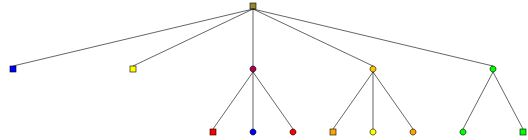
\includegraphics[width=300pt]{../images/experiment1_seq1_9.jpg}
    \caption{Experiment 1 with sequence 1}
    \label{Fig:experiment1_seq1}
\end{figure}

\begin{figure}[h!]
    \centering
    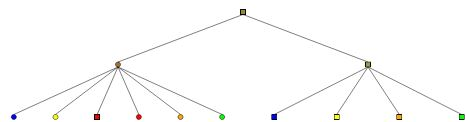
\includegraphics[width=300pt]{../images/experiment1_seq2_9.jpg}
    \caption{Experiment 1 with sequence 2}
    \label{Fig:experiment1_seq2}
\end{figure}

\subsection{Solution for Experiment 2}
Answers for this experiment are open. Here is one possible example. In an organization, people are grouped to different departments. Whenever new people come in, it will be decided which department they should join. Sometimes, several departments are merged to one and in some cases, one department might be broken down into several because of the newly added people. Attributes and values for this specific example could be:\\
\emph{experience,preference,age,gender,advantage\#\\
 extensive,relevant,none\#\\
 sales,management,logistics,nopreference\#\\
 female,male\#\\
 under,twenties,thirties,forties,above\#\\
 design,writing,communication\#\\} 

\subsection{Solution for Experiment 3}
There are usually three key steps to get the category utility of a certain classification. First, get the probability of each class. It is very straightforward. You just need to calculate the fraction of the number of objects in a certain class against the total number of objects. In this exercise, the number of objects in \emph{Class 1} is three, the same for \emph{class 2} and the total number of objects is six. Thus, the probability for $C_1$ is $$P(C_1)=\frac{3}{6}=0.5$$ and the probability for $C_2$ is $$P(C_2)=\frac{3}{6}=0.5$$ 

Second, get the expected number of attribute values that can be correctly guessed given a certain class. This is the conditional expectations (See Page 5). For each attribute value given \emph{Class 1}, we can get the following table \ref{tab:solexperiment3}:

\begin{table}[!ht]
 \ttabbox{\caption{}}
 {
 \centering
 \begin{tabular}{l l l l l l}\hline
 \textbf{ } & \textbf{ } & \textbf{Class 1 } & \textbf{} & \textbf{ } & \textbf{ } \\
 \textbf{A1} & \textbf{ } & \textbf{A2} & \textbf{ } & \textbf{A3} & \textbf{ } \\\hline
 \textbf{Green} & $({2}/{3})^2$ & \textbf{Ball} & $({3}/{3})^2$ & \textbf{Small} & $({2}/{3})^2$ \\
 \textbf{Red} & $({1}/{3})^2$ & \textbf{Square} & $(0/3)^2$ & \textbf{Large} & $({1}/{3})^2$ \\
 \textbf{Blue} & $(0/3)^2$ & -- & -- & -- & -- \\\hline
 \end{tabular}
 \label{tab:solexperiment3}}
 \end{table}
 The expected number of attribute values that can be correctly guessed given $C_1$ is: $$\sum_{i=1}^{3} \sum_{j=1}^{}P(A_i=V_{ij}\left|C_1\right.)^2=(\frac{2}{3})^2+(\frac{1}{3})^2+0+1+0+(\frac{2}{3})^2+(\frac{1}{3})^2=2.11$$
 
For each attribute value given \emph{Class 2}, we can get the following table \ref{tab:solexperiment31}:
  
  \begin{table}[!ht]
   \ttabbox{\caption{}}
   {
   \centering
   \begin{tabular}{l l l l l l}\hline
   \textbf{ } & \textbf{ } & \textbf{Class 1 } & \textbf{} & \textbf{ } & \textbf{ } \\
   \textbf{A1} & \textbf{ } & \textbf{A2} & \textbf{ } & \textbf{A3} & \textbf{ } \\\hline
   \textbf{Green} & $({1}/{3})^2$ & \textbf{Ball} & $({1}/{3})^2$ & \textbf{Small} & $({0}/{3})^2$ \\
   \textbf{Red} & $({0}/{3})^2$ & \textbf{Square} & $(2/3)^2$ & \textbf{Large} & $({3}/{3})^2$ \\
   \textbf{Blue} & $(2/3)^2$ & -- & -- & -- & -- \\\hline
   \end{tabular}
   \label{tab:solexperiment31}}
   \end{table}
The expected number of attribute values that can be correctly guessed given $C_2$ is: $$\sum_{i=1}^{3} \sum_{j=1}^{}P(A_i=V_{ij}\left|C_2\right.)^2=(\frac{1}{3})^2+0+(\frac{2}{3})^2+(\frac{1}{3})^2+(\frac{2}{3})^2+0+1=2.11$$

Last, get the expected number of attribute values that can be correctly guessed without any category knowledge. This is the unconditional expectations.
 \begin{table}[!ht]
   \ttabbox{\caption{}}
   {
   \centering
   \begin{tabular}{l l l l l l}\hline
   \textbf{A1} & \textbf{ } & \textbf{A2} & \textbf{ } & \textbf{A3} & \textbf{ } \\\hline
   \textbf{Green} & $({3}/{6})^2$ & \textbf{Ball} & $({4}/{6})^2$ & \textbf{Small} & $(2/6)^2$ \\
   \textbf{Red} & $(1/6)^2$ & \textbf{Square} & $(2/6)^2$ & \textbf{Large} & $(4/6)^2$ \\
   \textbf{Blue} & $(2/6)^2$ & -- & -- & -- & -- \\\hline
   \end{tabular}
   \label{tab:solexperiment32}}
   \end{table}
   
The expected number of attribute values that can be correctly guessed without any category information is: $$\sum_{i=1}^{3} \sum_{j=1}^{}P(A_i=V_{ij})^2=(\frac{3}{6})^2+(\frac{1}{6})^2+(\frac{2}{6})^2+(\frac{4}{6})^2+(\frac{2}{6})^2+(\frac{2}{6})^2+(\frac{4}{6})^2=1.5$$
Thus, we can get Category Utility for the current classification: $$CU=\frac{0.5\times(2.11-1.50)+0.5\times(2.11-1.50)}{2}=0.305$$

\subsection {Solution for Experiment 4}
If we go to the function \emph{undoLastStep()} in the file \emph{cluster.js}, we can see that there are four variables that hold the string representation of the cluster. These four variables are \emph{global\_backup\_text1, global\_backup\_text2, global\_backup\_text3 and global\_backup\_text4}. If you search any of them, you will see that they are defined in the very beginning of the \emph{cluster.js}. 

In order to see how the initial value is passed to the \emph{global\_backup\_text}, we need to search the first variable \emph{global\_backup\_text1}. Then you will find out that variable \emph{global\_backup\_text1} gets sting in the function \emph{addObjects()} and function \emph{addRandomObjects()}. Once the variable \emph{global\_backup\_text1} is updated, its previous string will be passed to the variable \emph{global\_backup\_text2} and so on so forth.

Then we go back to the function \emph{undoLastStep()} and now it is easy to know that if we want to undo the last step, we need to recover the values for the variables \emph{global\_backup\_text}. If we want to undo five steps, a new variable \emph{global\_backup\_text5} needs adding in this file. In order to solve this problem, there are four places that needs modifying in \emph{cluster.js}.
\begin{enumerate}[1)]
\item Add \emph{var global\_backup\_text5 = \lq\lq \rq\rq;} in the very beginning of \emph{cluster.js} to define it;
\item Add \emph{global\_backup\_text5 = global\_backup\_text4;} before the code \emph{global\_backup\_text4 = global\_backup\_text3;} in the beginning of the function \emph{addObjects()} to make sure that \emph{global\_backup\_text5} gets the value; 
\item Similar to the second. Add \emph{global\_backup\_text5 = global\_backup\_text4;} before the code \emph{global\_backup\_text4 = global\_backup\_text3;} in the middle of the function \emph{addRandomObjects()};
\item The last place that needs modifying is in the function \emph{undoLastStep()}. In the \emph{else} clause, add \emph{global\_backup\_text4 = global\_backup\_text5;} in front of the code \emph{global\_backup\_text4 = \lq\lq \rq\rq;} and change the code \emph{global\_backup\_text4 = \lq\lq \rq\rq;} to be \emph{global\_backup\_text5= \lq\lq \rq\rq;}
\item Restart the Conceptual Clustering simulation tool and the use the default setting. Add the objects more than five times and then try \lq\lq Undo Last Action \rq\rq button. You will be allowd to undo the last five steps instead of four.
\end{enumerate}
\appendix
%\include{handout}
\bibliographystyle{IEEEbib}
\bibliography{refs}

\end{document}
